\documentclass[12pt,oneside,bahasa]{book}
\usepackage{charter}
\usepackage[T1]{fontenc}
\usepackage[latin9]{inputenc}
\setcounter{secnumdepth}{3}
\setcounter{tocdepth}{3}
\usepackage{array}
\usepackage{longtable}
\usepackage{float}
\usepackage{varwidth}
\usepackage{graphicx}
\usepackage[a4paper]{geometry}
\geometry{verbose,tmargin=3cm,bmargin=3cm,lmargin=4cm,rmargin=3cm}
\usepackage{fancyhdr}
\pagestyle{fancy}
\usepackage{setspace}
\usepackage[authoryear]{natbib}
\onehalfspacing

\makeatletter

%%%%%%%%%%%%%%%%%%%%%%%%%%%%%% LyX specific LaTeX commands.
%% Because html converters don't know tabularnewline
\providecommand{\tabularnewline}{\\}
%% Variable width box for table cells
\newenvironment{cellvarwidth}[1][t]
    {\begin{varwidth}[#1]{\linewidth}}
    {\@finalstrut\@arstrutbox\end{varwidth}}

%%%%%%%%%%%%%%%%%%%%%%%%%%%%%% User specified LaTeX commands.
%% \renewcommand{\chapter}[1]{\chapter[#1]{\centering #1}}
\usepackage{titlesec}
\usepackage{graphicx}
\usepackage{indentfirst}
\titleformat{\chapter}[hang]
  {\normalfont\huge\bfseries\centering}{\thechapter.}{14pt}{\Huge\MakeUppercase}
%%-------------
\newcommand{\Judul}{Aplikasi \textit {Review} Artikel Ilmiah dengan metode \textit {Retrieval-Augmented Generation} Dan \textit {Langchain} }
\newcommand{\JudulInggris}{Scientific Article Review Application with Retrieval-Augmented Generation and Langchain method}
\newcommand{\Penulis}{Rafli Satya Dewanto}
\newcommand{\NPM}{51421208}
\newcommand{\NIRM}{98432324243}
\newcommand{\JenisTulisan}{Skripsi}
\newcommand{\Gelar}{Jenjang S1 / Setara Sarjana Muda}
\newcommand{\Fakultas}{Teknologi Industri}
\newcommand{\Faculty}{Industrial Technology}
\newcommand{\Jurusan}{Informatika}
\newcommand{\Major}{Informatics}
%%-------------
\newcommand{\Prodi}{Direktorat Program Diploma Tiga Teknologi Informasi}
\newcommand{\Tahun}{2025}
\newcommand{\Bulan}{Juli}
\newcommand{\Tanggal}{24}
\newcommand{\Kota}{JAKARTA}
%%-------------
\newcommand{\KataKunci}{\textit{Artifical Intelligence, Retrieval-Augmented Generation, Chatbot, Next.js, Gemini}}
\newcommand{\KeyWords}{Artifical Intelligence, Retrieval-Augmented Generation, Chatbot, Next.js, Gemini}
%%-------------
\newcommand{\KoordinatorPI}{Dr. Achmad Fahrurozi, S.Si., M.Si.}
%%-------------
\newcommand{\KetuaJurusan}{Prof. Dr. Lintang Yuniar Banowosari, S.Kom., M.Sc.}
\newcommand{\DosenPembimbingA}{Drs. Agus Sumin, MMSI.}
\newcommand{\DosenPembimbingB}{Dr. Ricky Agus T., S.T., S.Si., M.M.}
\newcommand{\KetuaPembimbing}{Prof. Dr. Lintang Yuniar Banowosari, S.Kom., M.Sc.}
\newcommand{\AnggotaPembimbingA}{Dr. Elfitrin Syahrul, ST., MT.}
\newcommand{\AnggotaPembimbingB}{Dr. Marliza Ganefi Gumay, S.Kom., MMSI}
%%------------
\newcommand{\KetuaUjian}{Dr. Ravi Ahmad Salim}
\newcommand{\SekUjian}{Prof. Dr. Wahyudi Priyono}
\newcommand{\AnggotaUjianA}{Prof. Dr. Lintang Yuniar Banowosari, S.Kom., M.Sc.}
\newcommand{\AnggotaUjianB}{Dr. Elfitrin Syahrul, ST., MT.}
\newcommand{\AnggotaUjianC}{Dr. Marliza Ganefi Gumay, S.Kom., MMSI}
%%-------------
\newcommand{\Ringkasan}{Tulis ringkasan skripsi, pi, atau apa dengan bahasa yang jelas, lugas dan menggambarkan secara singkat tulisan ini.  Sebaiknya tidak lebih dari 150 kata dan sudah menjelaskan dari permasalahan, pembahasan dan penutup.}
\newcommand{\JumlahPustaka}{50}
\newcommand{\JumlahHalaman}{89}
\newcommand{\JumlahHalamanDepan}{xiii}
\newcommand{\TahunPustaka}{1959-2024}
%%
%% Keterangan administratif sidang sarjana
%%
\newcommand{\TanggalSidang}{24 Juli 2025}
\newcommand{\TanggalLulus}{24 Juli 2025}
\newcommand{\TanggalSah}{}
\newcommand{\PejabatBagianSidang}{Dr. Edi Sukirman, S.Si., MM., M.I.Kom.}
\setlength{\headheight}{15pt}
%%-------------
%%
%%Untuk Kata pengantar
%%
\newcommand{\Rektor}{Prof. Dr. E.S. Margianti, SE., MM.}
\newcommand{\Dekan}{Prof. Dr. Ing. Adang Suhendra, S.Si, S.Kom., M.Sc.}
\newcommand{\KotaPenulis}{Depok}
\newcommand{\BlnThn}{24 Juli 2025}
%%-----------
%%-----------
% The following commands set the page numbers on the top right
% except in the beginning of chapters
%\lhead{}
%\chead{}
%\rhead{\thepage}
%\lfoot{}
%\cfoot{}
%\rfoot{}
%\renewcommand{\headrulewidth}{0pt}


\usepackage{tocloft}
% Mengatur judul Daftar Isi, Daftar Gambar, dan Daftar Tabel agar tetap rata tengah dengan ukuran default
\renewcommand{\cfttoctitlefont}{\hfill\Huge\bfseries}
\renewcommand{\cftloftitlefont}{\hfill\Huge\bfseries}
\renewcommand{\cftlottitlefont}{\hfill\Huge\bfseries}
\renewcommand{\cftaftertoctitle}{\hfill}
\renewcommand{\cftafterloftitle}{\hfill}
\renewcommand{\cftafterlottitle}{\hfill}
% Membuat daftar khusus untuk lampiran
\newlistof{appendices}{app}{Daftar Lampiran}
% Kode untuk mengatur judul Daftar Lampiran
\makeatletter
\renewcommand{\listofappendices}{%
  \chapter*{DAFTAR LAMPIRAN}%
  \@starttoc{app}%
}
\makeatother


\renewcommand{\cftchapleader}{\cftdotfill{\cftdotsep}}
\renewcommand{\cftsecleader}{\cftdotfill{\cftdotsep}}
\renewcommand{\cftsubsecleader}{\cftdotfill{\cftdotsep}}



% Define custom page numbering style
\usepackage{fancyhdr}
\newcommand{\appendixpagenumbering}{
    \renewcommand{\thepage}{L-\arabic{page}}
}


% Mengatur header dan footer
\fancypagestyle{romanstyle}{
    \fancyhf{}
    \fancyfoot[C]{\thepage} % Nomor halaman di tengah bawah
    \renewcommand{\headrulewidth}{0pt} % Hapus garis header
    \renewcommand{\footrulewidth}{0pt} % Hapus garis footer
}

\fancypagestyle{arabicstyle}{
    \fancyhf{}
    \fancyhead[R]{\thepage} % Nomor halaman di kanan atas
    \renewcommand{\headrulewidth}{0pt} % Hapus garis header
    \renewcommand{\footrulewidth}{0pt} % Hapus garis footer
}

\fancypagestyle{appendixstyle}{
    \fancyhf{}
    \fancyfoot[C]{\thepage} % Nomor halaman di tengah bawah
    \renewcommand{\headrulewidth}{0pt} % Hapus garis header
    \renewcommand{\footrulewidth}{0pt} % Hapus garis footer
}

\makeatother

\usepackage{babel}
\usepackage{listings}
\renewcommand{\lstlistingname}{Listing}

\begin{document}
\hyphenation {meng-hi-lang-kan pa-ling li-sen-si ge-ne-ral di-tam-bah
             me-nge-nai da-pat kom-pu-ter ke-dua di-ban-ding-kan
             de-ngan sa-dar meng-aki-bat-kan ber-da-sar-kan
             ke-ti-dak-ha-ti-ha-ti-an me-la-ku-kan di-be-ri-kan
             mem-ba-tasi pe-ne-kan-an ber-ka-it-an me-nya-lin
             me-nye-bar-lu-as-kan ber-asal men-dis-tri-bu-si-kan
             ma-na-kah meng-ha-sil-kan peng-ubah-an awal di-be-ri-kan
             meng-hor-mati mi-sal-nya mi-sal pu-blik pro-ses 
             meng-atur ke-cen-de-rung-an di-ra-ha-sia-kan 
             pa-ten pe-ne-ri-ma hu-kum di-nya-ta-kan wa-lau-pun
             mes-ki-pun di-se-rah-kan un-dang-un-dang ada-nya
             per-lin-dung-an meng-u-bah mem-pu-nyai ter-da-pat
             pe-mro-gram-an ini-lah ke-ta-kut-an men-da-pat-kan
             re-pu-blik in-do-ne-sia pe-ngem-bang-an ke-nya-ta-an 
             pan-dang-an di-ka-te-go-ri-kan ke-sim-pul-an 
             ka-lang-an se-pan-jang pe-ner-je-mah-an ingin-kan
             di-im-ple-men-ta-si-kan pen-ting ke-ingin-an
             meng-emu-la-si de-fi-ni-si-kan sam-ping apli-ka-si
             me-nyim-pan ma-na-ger kon-fi-gu-ra-si user ha-lam-an
             per-mo-hon-an sa-ngat suatu ma-nu-al me-na-ngani 
             di-li-hat du-kung-an ter-je-mah-an-nya ter-je-mah-an 
             ling-kung-an di-sim-pan meng-u-sa-ha-kan sa-ngat-lah
             me-re-pre-sen-ta-si-kan pe-nyim-pan-an se-ring
             spa-nyol me-nying-kat-nya apli-ka-si-nya
             ke-nya-ta-an-nya me-nge-lu-ar-kan desk-top in-ter-face
             in-ter-net ke-ku-rang-an me-mung-kin-kan fol-der 
             me-nye-ret-nya meng-u-bah-nya me-ngor-ban-kan
             peng-a-tur-an pe-nam-pil-an di-ki-rim-kan 
             meng-en-krip-si-nya pi-lih per-so-nal-iza-ti-on 
             pre-fer-en-si meng-kon-fi-gu-ra-si-kan-nya di-tam-pil-kan
             lam-pir-an be-be-ra-pa meng-a-cu pe-ngi-rim peng-a-tur-an 
             chall-enge meng-o-ten-ti-fi-ka-si me-nyim-pan-nya 
	     me-nye-dia-kan di-kem-bang-kan meng-u-bah pe-rang-kat 
	     send-mail di-gu-na-kan plat-form mem-for-mat ko-or-di-na-tor 
	     meng-gu-na-kan me-ngua-sai mem-bu-tuh-kan root line 
	     di-se-suai-kan me-ngi-rim-kan ope-ra-si se-ring-ka-li 
             di-gi-tal mem-ban-ding-kan meng-a-na-li-sa fe-no-me-na 
             peng-o-lah-an usa-ha pe-mi-lih-an fa-si-li-tas me-mo-ri 
             ke-hi-dup-an}
 
\sloppy 
\thispagestyle{empty}

\addcontentsline{toc}{chapter}{HALAMAN JUDUL}

\pagenumbering{roman}
\pagestyle{romanstyle}

\vspace*{10mm}

\begin{center}
{\large\textbf{UNIVERSITAS GUNADARMA}}{\large\par}
\par\end{center}

\begin{center}
{\large\textbf{FAKULTAS \MakeUppercase{\Fakultas}}}{\large\par}
\par\end{center}

\vspace*{10mm}

\begin{center}

\includegraphics[width=55mm]{images/gundarlogo.png}
\par\end{center}

\vspace*{3mm}

\begin{center}
{\Large\textbf{SKRIPSI}}{\Large\par}
\par\end{center}

\vspace*{7mm}

\begin{center}
\begin{tabular}{|>{\centering}m{13.5cm}|}
\hline 
\centering{}~~\tabularnewline
\centering{}\textbf{\MakeUppercase{\Judul}}\tabularnewline
~~\tabularnewline
\centering{}%
\begin{tabular}{lcl}
Nama & : & \Penulis\tabularnewline
NPM & : & \NPM\tabularnewline
Fakultas & : & \Fakultas\tabularnewline
Program Studi & : & \Jurusan\tabularnewline
Dosen Pembimbing 1 & : & \DosenPembimbingA\tabularnewline
Dosen Pembimbing 2 & : & \DosenPembimbingB\tabularnewline
\end{tabular}\tabularnewline
~~\tabularnewline
\hline 
\end{tabular}
\par\end{center}

 \vspace{7mm}

\begin{center}
\begin{tabular}{c}
\begin{cellvarwidth}[t]
\centering
\textbf{Diajukan Guna Melengkapi Sebagian Syarat Dalam Mencapai }

\textbf{Gelar Setara Sarjana Strata Satu (S1)}
\end{cellvarwidth}\tabularnewline
\textbf{\Kota}\tabularnewline
\textbf{\Tahun}\tabularnewline
\end{tabular}
\par\end{center}

\chapter*{{\huge PERNYATAAN ORISINALITAS DAN PUBLIKASI}}

\begin{singlespace}
\addcontentsline{toc}{chapter}{PERNYATAAN ORISINALITAS DAN PUBLIKASI}
\thispagestyle{romanstyle}

Saya yang bertanda tangan di bawah ini,

\vspace*{10mm}

\hspace{-6pt}%
\begin{tabular}{>{\raggedright}p{30mm}c>{\raggedright}p{0.66\textwidth}}
Nama & : & \Penulis\tabularnewline
NPM & : & \NPM\tabularnewline
Judul PI & : & \MakeUppercase{\Judul}\tabularnewline
Tanggal Sidang & : & \TanggalSidang\tabularnewline
Tanggal Lulus & : & \TanggalLulus\tabularnewline
\end{tabular}

\vspace*{10mm}

\noindent menyatakan bahwa tulisan ini adalah merupakan hasil karya
saya sendiri dan dapat dipublikasikan sepenuhnya oleh Universitas
Gunadarma. Segala kutipan dalam bentuk apa pun telah mengikuti kaidah
dan etika yang berlaku. Semua hak cipta dari logo serta produk yang
disebut dalam buku ini adalah milik masing-masing pemegang haknya,
kecuali disebutkan lain. Mengenai isi dan tulisan merupakan tanggung
jawab Penulis, bukan Universitas Gunadarma.

Demikianlah pernyataan ini dibuat dengan sebenarnya dan dengan penuh
kesadaran.

\vspace*{15mm}
\end{singlespace}

\begin{flushright}
\begin{tabular}{c}
\KotaPenulis, \  \Tanggal\ \Bulan\ \Tahun\tabularnewline
\vspace*{25mm}\tabularnewline
\Penulis\tabularnewline
\end{tabular}
\par\end{flushright}

\chapter*{{\huge LEMBAR PENGESAHAN}}

\addcontentsline{toc}{chapter}{LEMBAR PENGESAHAN}

\begin{center}
\begin{tabular}{|c|ll|c|}
\multicolumn{4}{c}{\textbf{KOMISI PEMBIMBING}}\tabularnewline
\hline 
\textbf{NO} & \multicolumn{2}{c|}{\textbf{NAMA}} & \textbf{KEDUDUKAN}\tabularnewline
\hline 
1. & \KetuaPembimbing &  & Ketua\tabularnewline
\hline 
2. & \AnggotaPembimbingA &  & Anggota\tabularnewline
\hline 
3. & \AnggotaPembimbingB &  & Anggota\tabularnewline
\hline 
\end{tabular}
\par\end{center}

\begin{center}
\begin{tabular}{|c|ll|c|}
\multicolumn{4}{c}{\textbf{PANITIA UJIAN}}\tabularnewline
\hline 
\textbf{NO} & \multicolumn{2}{c|}{\textbf{NAMA}} & \textbf{KEDUDUKAN}\tabularnewline
\hline 
1. & \KetuaUjian &  & Ketua\tabularnewline
\hline 
2. & \SekUjian &  & Sekretaris\tabularnewline
\hline 
3. & \AnggotaUjianA &  & Anggota\tabularnewline
\hline 
4. & \AnggotaUjianB &  & Anggota\tabularnewline
\hline 
5. & \AnggotaUjianC &  & Anggota\tabularnewline
\hline 
\end{tabular}
\par\end{center}

\begin{center}
\vspace*{5mm}
\par\end{center}

\begin{center}
\begin{tabular}{ccc}
\multicolumn{3}{c}{\textbf{Mengetahui,}}\tabularnewline
\multicolumn{3}{c}{\textbf{\vspace*{5mm}}}\tabularnewline
\textbf{Dosen Pembimbing} &  & \textbf{Bagian Sidang Ujian}\tabularnewline
\textbf{\vspace*{10mm}} &  & \textbf{\vspace*{10mm}}\tabularnewline
\textbf{(\DosenPembimbingB)} &  & \textbf{(\KoordinatorPI)}\tabularnewline
\end{tabular}
\par\end{center}

\chapter*{ABSTRAK}

\begin{singlespace}
\addcontentsline{toc}{chapter}{ABSTRAK}

\noindent\Penulis. \NPM

\noindent\MakeUppercase{\Judul} \\
Skripsi, Fakultas \Fakultas, Program Studi \Jurusan, Universitas
Gunadarma, \Tahun

\noindent Kata Kunci : \KataKunci

\medskip{}

\noindent (\JumlahHalamanDepan \ + \JumlahHalaman \ + lampiran)

\bigskip{}

\emph{Deepfake}, teknologi yang memanfaatkan \emph{machine learning}
untuk memanipulasi video dan gambar, telah menjadi tantangan besar
dalam beberapa tahun terakhir.

\bigskip{}

\noindent Daftar Pustaka (\TahunPustaka)
\end{singlespace}

\chapter*{ABSTRACT}

\begin{singlespace}
\addcontentsline{toc}{chapter}{ABSTRACT}

\noindent\Penulis. \NPM

\noindent\MakeUppercase{\JudulInggris} \\
Thesis, Faculty of \Faculty, \Major\ Study Program, Gunadarma University,
\Tahun

\noindent Keywords : \KeyWords

\medskip{}

\noindent (\JumlahHalamanDepan \ + \JumlahHalaman \ + attachment)

\bigskip{}

Deepfake, a technology that uses machine learning to manipulate videos
and images, has become a major challenge in recent years.

\bigskip{}

\noindent Bibliography (\TahunPustaka)
\end{singlespace}

\chapter*{KATA PENGANTAR}

\thispagestyle{plain}
\addcontentsline{toc}{chapter}{KATA PENGANTAR}

Puji syukur ke hadirat Tuhan Yang Maha Esa atas segala rahmat dan
karunia-Nya, serta doa dan dorongan dari berbagai pihak, sehingga
skripsi yang berjudul ``\Judul'' dapat diselesaikan dengan baik.

Penyusunan skripsi ini merupakan salah satu syarat untuk mencapai
jenjang Setara Sarjana Strata Satu (S1) pada Program Studi Informatika,
Fakultas Teknologi Industri, Universitas Gunadarma.

Walaupun dalam penyusunannya menemui berbagai kendala, berkat bantuan
dan dorongan dari berbagai pihak, skripsi ini dapat diselesaikan dengan
baik. Penulis ingin mengucapkan terima kasih kepada: 
\begin{enumerate}
\item \Rektor, selaku Rektor Universitas Gunadarma.
\item \Dekan, selaku Dekan Fakultas Teknologi Industri, Universitas Gunadarma.
\item \KetuaJurusan , selaku Ketua Program Studi \Jurusan.
\item \KoordinatorPI, selaku Kepala Subbagian Sidang PI Fakultas Teknologi
Industri.
\item \DosenPembimbingA\ dan \DosenPembimbingB, sebagai Dosen Pembimbing
yang di tengah-tengah aktivitas dan kesibukannya telah membimbing
dan memberikan dorongan serta dukungan, sehingga penulisan ini dapat
diselesaikan.
\item Seluruh rekan 4IA01 di Universitas Gunadarma yang telah banyak
membantu serta memberi semangat selama proses penulisan. 
\item Semua pihak yang tidak bisa disebutkan yang telah membantu penyelesaian
skripsi ini, diucapkan juga terima kasih atas segala bantuan dan sarannya. 
\end{enumerate}
\indent

Sebagai manusia biasa yang tidak luput dari kesalahan, penulis menyadari
bahwa skripsi ini masih jauh dari sempurna dan memiliki banyak kekurangan.
Oleh karena itu, penulis dengan terbuka menerima kritik dan saran
yang bersifat membangun demi perbaikan di masa yang akan datang. Semoga
skripsi ini dapat memberikan manfaat bagi para pembaca dan menjadi
kontribusi kecil bagi kemajuan ilmu pengetahuan.

\begin{singlespace}
\vspace*{15mm}


\end{singlespace}\begin{flushright}
\begin{tabular}{c}
\KotaPenulis, \BlnThn\vspace{10pt}\tabularnewline
Penulis\tabularnewline
\vspace*{25mm}\tabularnewline
\Penulis\tabularnewline
\end{tabular}
\par\end{flushright}

\clearpage
\phantomsection 
\vspace*{7mm}

\thispagestyle{plain}
\addcontentsline{toc}{chapter}{DAFTAR ISI}
\renewcommand\contentsname{DAFTAR ISI}

\tableofcontents{}

\clearpage
\phantomsection 
\vspace*{7mm}

\thispagestyle{plain}
\addcontentsline{toc}{chapter}{DAFTAR TABEL}
\renewcommand\listtablename{DAFTAR TABEL}

\listoftables

\clearpage
\phantomsection 
\vspace*{7mm}

\thispagestyle{plain}
\addcontentsline{toc}{chapter}{DAFTAR GAMBAR}
\renewcommand\listfigurename{DAFTAR GAMBAR}

\listoffigures

\clearpage
\phantomsection 

\thispagestyle{plain}
\addcontentsline{toc}{chapter}{DAFTAR LAMPIRAN}
\listofappendices
\chapter{PENDAHULUAN}

\setcounter{page}{1}
\pagenumbering{arabic}
\thispagestyle{plain}
\pagestyle{arabicstyle}

\section{Latar Belakang Masalah}

Mahasiswa, terutama yang bukan penutur asli bahasa Inggris, sering menghadapi tantangan dalam memahami teks akademik berbahasa Inggris. Kesulitan ini disebabkan oleh kompleksitas struktur kalimat, penggunaan kosakata teknis, dan gaya penulisan yang formal. Penelitian oleh~\cite{Dardjito} menunjukkan bahwa mahasiswa di Indonesia sering merasa cemas dan kurang percaya diri saat membaca jurnal akademik dalam bahasa Inggris, yang berdampak negatif pada keterlibatan mereka dalam proses pembelajaran dan penelitian. Kesulitan ini juga dapat menghambat kemampuan mereka untuk mengembangkan pemikiran kritis dan berkontribusi dalam diskusi ilmiah di bidang studi mereka.

Sebagai solusi terhadap tantangan tersebut, pemanfaatan Artificial Intelligence (AI) dapat secara signifikan meningkatkan pengalaman dan hasil mahasiswa dalam penulisan research paper melalui beberapa mekanisme yang bermanfaat. AI-powered writing tools, seperti pemeriksa tata bahasa dan asisten gaya, memberikan feedback real-time tentang kualitas tulisan, membantu mahasiswa menyempurnakan tata bahasa dan sintaksis mereka untuk menghasilkan teks yang lebih jelas dan koheren \citep{kong2024pedagogical,nazari2021application}. Dengan menggabungkan alat tersebut ke dalam proses penulisan mereka, mahasiswa tidak hanya dapat meningkatkan aspek teknis dari pekerjaan mereka tetapi juga meningkatkan kepercayaan diri mereka dalam menyusun teks akademik \citep{nazari2021application}.

Peran AI meluas melampaui mekanisme bahasa. AI juga dapat membantu dalam melakukan tinjauan literatur dengan cepat meringkas penelitian yang ada dan mengidentifikasi sumber-sumber yang relevan, yang menyederhanakan proses penelitian akademik \citep{gupta2024artificial}. Misalnya, alat AI dapat menganalisis volume besar literatur akademik untuk menyajikan ringkasan singkat, membantu mahasiswa dalam mengumpulkan dan mensintesis informasi yang diperlukan untuk paper mereka secara efisien \citep{bulante2024ai}. Integrasi AI ini tidak hanya meningkatkan efisiensi penelitian tetapi juga membantu mahasiswa mengembangkan kemampuan membaca kritis dan analitis dengan mendorong mereka untuk terlibat dengan konten yang telah disintesis.

Penggabungan Retrieval-Augmented Generation dalam aplikasi chatbot berfungsi untuk memperluas batasan yang melekat pada model generasi konvensional. LLM tradisional sering kali kesulitan dengan akurasi faktual, terutama ketika ditanyai tentang informasi yang spesifik atau dinamis \citep{wang2024mememo,lewis2020retrieval}. Teknik RAG secara efektif mengatasi masalah ini dengan memungkinkan model mengakses dan menggabungkan pengetahuan real-time dari database eksternal, memastikan bahwa respons tidak hanya relevan secara kontekstual tetapi juga akurat dan koheren \citep{lewis2020retrieval}.

Dengan adanya aplikasi ini, mahasiswa dapat berinteraksi secara aktif dengan isi jurnal, bukan hanya membaca pasif, sehingga meningkatkan keterlibatan dan pemahaman akademik mereka. Aplikasi ini bukan bertujuan untuk menggantikan proses berpikir kritis, tetapi mendukung mahasiswa menjadi lebih mandiri dan efisien dalam memahami literatur dan mengelola catatan pribadi mereka. Dengan demikian, pengembangan aplikasi chatbot ini diharapkan mampu menjadi alat bantu yang efektif bagi mahasiswa dalam memahami isi jurnal, mencatat poin penting, dan menyusun sitasi dengan lebih efisien

\section{Rumusan Masalah}
Dalam penulisan ini terdapat beberapa rumusan masalah yang penulis akan bahas, diantaranya:
\begin{enumerate}
  \item Bagaimana merancang dan mengembangkan aplikasi chatbot yang dapat membantu mahasiswa memahami isi jurnal akademik berbahasa Inggris yang kompleks?
        \raggedright
  \item Bagaimana pemanfaatan metode Retrieval-Augmented Generation (RAG) dapat meningkatkan akurasi dan relevansi jawaban chatbot terhadap pertanyaan terkait isi jurnal?
  \item Bagaimana integrasi teknologi Langchain dapat mendukung kemampuan chatbot dalam berinteraksi secara kontekstual dan memberikan pengalaman yang lebih adaptif kepada pengguna?
  \item Bagaimana aplikasi ini dapat membantu mahasiswa dalam membuat sitasi otomatis dengan berbagai gaya referensi?
  \item Bagaimana aplikasi ini dapat menyediakan fitur anotasi PDF sebagai catatan pribadi mahasiswa dalam proses riset?
\end{enumerate}

\section{Ruang Lingkup}

Batasan-batasan tersebut adalah sebagai berikut.
\begin{enumerate}
  \item Citra
\end{enumerate}

\section{Tujuan Penelitian}

Tujuan penelitian yang akan dibahas adalah sebagai berikut.
\begin{enumerate}
  \item lorem ipsum
\end{enumerate}

\section{Sistematika Penulisan}

Sistematika yang digunakan dalam penulisan ini mencakup beberapa bagian
penting, di antaranya:
\begin{enumerate}
  \item PENDAHULUAN

        Bab ini berisi pendahuluan yang menguraikan latar belakang masalah
        yang melandasi pemilihan topik penelitian, didukung oleh data relevan
        dan perbandingan dengan penelitian terdahulu, yang menyoroti kelemahan
        atau perbedaan pendekatan. Ruang lingkup penelitian dibatasi secara
        jelas untuk fokus pada persoalan yang dikaji. Tujuan penelitian ini
        adalah untuk menjawab masalah penelitian dan menghasilkan luaran yang
        diharapkan. Sistematika penulisan laporan skripsi ini akan disusun
        secara naratif, dimulai dari bab pendahuluan yang menguraikan konteks
        penelitian, diikuti oleh tinjauan pustaka yang membahas landasan teoretis,
        metodologi penelitian yang menjelaskan pendekatan dan teknik pengumpulan
        data, hasil penelitian dan pembahasan yang menganalisis temuan, hingga
        kesimpulan dan saran yang merangkum hasil penelitian dan implikasinya.
  \item TINJAUAN PUSTAKA

        Bab ini merupakan tinjauan pustaka yang disusun untuk memberikan landasan
        teoretis dan empiris yang kokoh dalam mendukung pendekatan pemecahan
        masalah yang diusulkan. Bab ini menguraikan secara komprehensif hasil
        penelitian sejenis yang relevan dengan tema yang dipilih, dengan menekankan
        pada kontribusi penelitian-penelitian tersebut terhadap pengembangan
        kerangka teoretis dan metodologis penelitian ini. Selain itu, tinjauan
        pustaka ini juga berfungsi untuk memperkuat argumentasi penelitian
        dengan menunjukkan bukti-bukti empiris dari penelitian sebelumnya,
        serta mengidentifikasi celah penelitian yang akan diisi oleh penelitian
        ini. Tinjauan pustaka ini tidak hanya merangkum literatur yang ada,
        tetapi juga menganalisis dan mensintesisnya untuk membangun dasar
        yang kuat bagi penelitian ini.
  \item HASIL DAN PEMBAHASAN

        Bab ini menyajikan hasil penelitian yang diperoleh, disertai dengan
        analisis mendalam untuk menjawab tujuan penelitian yang telah ditetapkan.
        Pada kasus penelitian yang menghasilkan rancangan, bab ini memuat
        deskripsi rinci hasil rancangan tersebut, termasuk evaluasi komprehensif
        terhadap kelebihan dan keterbatasan yang teridentifikasi. Analisis
        ini dilakukan secara sistematis dan objektif, dengan mengacu pada
        kerangka teoretis dan metodologis yang telah ditetapkan sebelumnya.
  \item PENUTUP

        Bagian penutup ini terdiri dari kesimpulan, yang merangkum jawaban
        atas masalah penelitian berdasarkan temuan yang diperoleh, dan saran,
        yang mengusulkan pengembangan lebih lanjut dari hasil penelitian yang
        telah dipaparkan dalam kesimpulan.
\end{enumerate}
\chapter{TINJAUAN PUSTAKA}

\section{Kajian Penelitian}

Penelitian yang dilakukan dalam pembuatan sistem deteksi, ekstraksi,
dan penghitungan luas batu ginjal menggunakan gabungan YOLO dan pengolahan
citra ini dilakukan dengan mempelajari penelitian-penelitian yang
sudah dilakukan oleh peneliti terdahulu. Penelitian yang dikaji mengutamakan
penelitian seputar deteksi batu ginjal dengan menggunakan model algoritma
\emph{machine learning} You Only Look Once (YOLO) dan perhitungan
luas batu ginjal tersebut dengan pendekatan pengolahan citra.

\subsection{\emph{Real-Time Object Detection in Medical Imaging Using YOLO Models
for Kidney Stone Detection} \citep{billah12s}}

Penelitian ini membahas deteksi batu ginjal secara real-time menggunakan
model YOLOv8 dan YOLOv10 pada citra CT \emph{scan} medis.

\vspace{20pt}

Tabel 2.1 menjelaskan secara ringkas penelitian-penelitian terdahulu
terhadap deteksi, ekstraksi, dan penghitungan luas batu ginjal menggunakan
gabungan YOLO dan pengolahan citra yang sudah dikaji.

\vspace{-10pt}

\begin{table}[H]
\begin{spacing}{0}
\caption{Rangkuman Penelitian Terdahulu}
\end{spacing}
\end{table}

\vspace{-20pt}
\begin{center}
\begin{longtable}[c]{|>{\centering}m{0.5cm}|>{\raggedright}p{3cm}|>{\raggedright}p{3.5cm}|>{\raggedright}p{5cm}|}
\hline 
\centering{}{\footnotesize\textbf{No}} & \centering{}{\footnotesize\textbf{Peneliti}} & \centering{}{\footnotesize\textbf{Judul Penelitian}} & {\footnotesize\textbf{Hasil}}\tabularnewline
\endfirsthead
\hline 
\centering{}{\footnotesize\textbf{No}} & \centering{}{\footnotesize\textbf{Peneliti}} & \centering{}{\footnotesize\textbf{Judul Penelitian}} & {\footnotesize\textbf{Hasil}}\tabularnewline
\endhead
\hline 
{\footnotesize 1} & {\footnotesize\citealp{billah12s}} & {\footnotesize\emph{Real-Time Object Detection in Medical Imaging
Using YOLO Models for Kidney Stone Detection}} & {\footnotesize Hasil menunjukkan bahwa YOLOv10 unggul dalam akurasi
(91\% dibandingkan 88\% untuk YOLOv8)}\tabularnewline
\hline 
 &  &  & \tabularnewline
\hline 
 &  &  & \tabularnewline
\hline 
 &  &  & \tabularnewline
\hline 
 &  &  & \tabularnewline
\hline 
 &  &  & \tabularnewline
\hline 
 &  &  & \tabularnewline
\hline 
\end{longtable}
\par\end{center}

\vspace{-40pt}

\section{\emph{Flowchart}}

Secara formal, \emph{flowchart} adalah representasi diagramatik dari
langkah-langkah suatu algoritma. Dalam \emph{flowchart}, digunakan
kotak dengan bentuk berbeda untuk menunjukkan jenis operasi yang berbeda.
Kotak-kotak ini kemudian dihubungkan oleh garis dengan panah yang
menunjukkan aliran atau arah yang harus diikuti untuk mengetahui langkah
selanjutnya. Garis penghubung ini dikenal sebagai garis alir (\emph{flow
line}).

\emph{Flowchart} program adalah alat yang sangat berguna dalam pengembangan
program. Pertama, kesalahan atau kelalaian dapat lebih mudah dideteksi
dari \emph{flowchart} program daripada dari program itu sendiri karena
\emph{flowchart} program adalah representasi bergambar dari logika
program. Kedua, \emph{flowchart} program dapat diikuti dengan mudah
dan cepat. Ketiga, ini berfungsi sebagai dokumentasi, yang dapat sangat
membantu jika diperlukan modifikasi program di masa mendatang.

\emph{Flowchart} dapat digunakan untuk menunjukkan urutan langkah
untuk melakukan pekerjaan apa pun. Rangkaian operasi sederhana yang
melibatkan penerimaan \emph{input}, pelaksanaan operasi aritmetika
pada \emph{input}, dan menampilkannya kepada pengguna dapat digunakan
untuk menunjukkan struktur logika sekuensial dari suatu program \citep{chaudhuri2020flowchart}.

\begin{table}[H]
\caption{Simbol Standar \emph{Flowchart} Program}

\centering{}(Sumber: \citealp{chaudhuri2020flowchart})
\end{table}

\vspace{-25pt}

\begin{longtable}[c]{|>{\centering}m{4cm}|>{\raggedright}m{9.5cm}|}
\hline 
\textbf{Simbol} & \centering{}\textbf{Keterangan}\tabularnewline
\hline 
\endfirsthead
\hline 
\textbf{Simbol} & \centering{}\textbf{Keterangan}\tabularnewline
\hline 
\endhead
\hline 
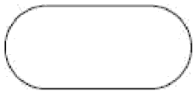
\includegraphics[totalheight=1.3cm]{images/flow_terminal} & Terminal:

Digunakan untuk menunjukkan awal dan akhir dari rangkaian proses yang
berhubungan dengan komputer.\tabularnewline
\hline 
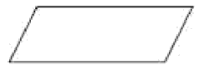
\includegraphics[totalheight=1cm]{images/flow_io} & \emph{Input/Output} (Masukan/Keluaran):

Digunakan untuk menunjukkan operasi \emph{input/output} apa pun.\tabularnewline
\hline 
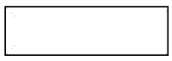
\includegraphics[totalheight=1cm]{images/flow_proc} & Pemrosesan Komputer (\emph{Computer Processing}):

Digunakan untuk menunjukkan pemrosesan apa pun yang dilakukan oleh
sistem komputer.\tabularnewline
\hline 
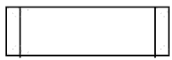
\includegraphics[totalheight=1cm]{images/flow_predproc} & Pemrosesan Tertentu (\emph{Predefined processing}):

Digunakan untuk menunjukkan proses apa pun yang tidak didefinisikan
secara khusus dalam \emph{flowchart}.\tabularnewline
\hline 
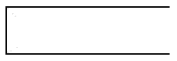
\includegraphics[totalheight=1cm]{images/flow_comm} & Komentar (\emph{Comment}):

Digunakan untuk menulis pernyataan penjelasan yang diperlukan untuk
memperjelas sesuatu.\tabularnewline
\hline 
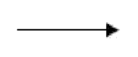
\includegraphics[totalheight=1.5cm]{images/flow_fl} & Garis Alir (\emph{Flow line}):

Digunakan untuk menghubungkan simbol-simbol \emph{flowchart}.\tabularnewline
\hline 
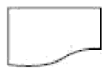
\includegraphics[totalheight=1.5cm]{images/flow_docio} & Masukan/Keluaran Dokumen (\emph{Document Input/Output}):

Digunakan ketika \emph{input} berasal dari dokumen dan \emph{output}
menuju ke dokumen.\tabularnewline
\hline 
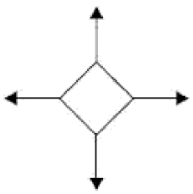
\includegraphics[totalheight=1.8cm]{images/flow_deci} & Keputusan (\emph{Decision}):

Digunakan untuk menunjukkan titik mana pun dalam proses di mana keputusan
harus dibuat untuk menentukan tindakan selanjutnya.\tabularnewline
\hline 
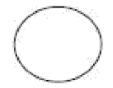
\includegraphics[totalheight=1.7cm]{images/flow_oncon} & Penghubung Halaman (\emph{On-page Connector}):

Digunakan untuk menghubungkan bagian-bagian \emph{flowchart} yang
dilanjutkan pada halaman yang sama.\tabularnewline
\hline 

\includegraphics[totalheight=1.9cm]{images/flow_offcon} & Penghubung Antar-Halaman (\emph{Off-page Connector}):

Digunakan untuk menghubungkan bagian-bagian \emph{flowchart} yang
dilanjutkan ke halaman yang terpisah.\tabularnewline
\hline 
\end{longtable}
\chapter{METODE PENELITIAN}

\section{Spesifikasi Perangkat Keras}

Tabel 3.1 menunjukkan informasi lengkap seluruh perangkat keras yang
dipergunakan dalam penelitian ini.

\begin{table}[H]
  \caption{Spesifikasi Perangkat Keras yang Digunakan}

  \centering{}%
  \begin{tabular}{|l|l|}
    \hline
    \textbf{Komponen} & \textbf{Nama}\tabularnewline
    \hline
    \hline
    CPU               & Apple Chip M1\tabularnewline
    \hline
    GPU               & Apple Chip M1\tabularnewline
    \hline
    RAM               & 8GB\tabularnewline
    \hline
    \emph{Chipset}    & M1\tabularnewline
    \hline
    SSD               & 256GB\tabularnewline
    \hline
  \end{tabular}
\end{table}


\section{Spesifikasi Perangkat Lunak}

Tabel 3.2 menunjukkan informasi lengkap mengenai seluruh perangkat
lunak yang dipergunakan dalam penelitian ini.

\begin{table}[H]
  \caption{Spesifikasi Perangkat Lunak yang Digunakan}

  \centering{}%
  \begin{tabular}{|l|l|}
    \hline
    \textbf{Aplikasi}          & \textbf{Nama}\tabularnewline
    \hline
    \hline
    OS                         & Macintosh\tabularnewline
    \hline
    \emph{Virtual Environment} & \emph{Node Package Mananger}\tabularnewline
    \hline
    Bahasa Pemrograman         & \emph{TypeScript}\tabularnewline
    \hline
    Editor Teks                & \emph{VS Code}\tabularnewline
    \hline
    \emph{Terminal Emulator}   & \emph{Ghostty}\tabularnewline
    \hline
    \emph{Framework}           & \emph{Next.js}\tabularnewline
    \hline
    Penelusur Web              & \emph{Arc}\tabularnewline
    \hline
    \emph{Version Control}     & \emph{Git}\tabularnewline
    \hline
  \end{tabular}
\end{table}
\section{Analisis Kebutuhan}
Tahap awal ini dilakukan untuk mengidentifikasi kebutuhan pengguna dan sistem. Fokus utama adalah permasalahan yang dihadapi mahasiswa dalam memahami jurnal ilmiah, serta fitur yang diperlukan seperti tanya jawab berbasis dokumen, sitasi otomatis, dan anotasi PDF. Dari tahap ini diturunkan kebutuhan fungsional dan non-fungsional sebagai dasar pengembangan sistem.

\section{Tools dan Peralatan Penelitian}
Penelitian ini menggunakan kombinasi perangkat lunak dan layanan AI untuk membangun sistem. Beberapa alat dan teknologi utama meliputi:
\begin{itemize}
  \item \textbf{Bahasa pemrograman:} JavaScript (Node.js), TypeScript (Next.js).
  \item \textbf{Framework AI:} Langchain untuk integrasi LLM dan retrieval.
  \item \textbf{Model AI:} OpenAI GPT-4 melalui API resmi.
  \item \textbf{Basis data:} Supabase PostgreSQL untuk data struktural, dan Chroma sebagai vektor store.
  \item \textbf{\emph{Tools} pendukung}:
        \begin{itemize}
          \item \emph{Postman} untuk API \emph{testing}.
          \item \emph{Visual Studio Code} untuk \emph{development}.
          \item \emph{GitHub} untuk kontrol versi.
        \end{itemize}
\end{itemize}

\section{Perancangan Sistem}
Pada tahap desain, dilakukan:
\begin{itemize}
  \item Perancangan arsitektur sistem yang mengintegrasikan \textit{front-end}, \textit{back-end}, dan layanan AI eksternal.
  \item Perancangan alur proses RAG menggunakan \textit{Langchain}, yang menghubungkan retriever, dokumentasi, dan model LLM.
  \item Desain tampilan antarmuka pengguna (\textit{user interface}) untuk memudahkan mahasiswa dalam mengunggah artikel ilmiah, melakukan interaksi tanya-jawab, membuat sitasi, dan memberi anotasi pada PDF.\@
  \item Perancangan struktur database menggunakan \textit{PostgreSQL} dan \textit{Redis} untuk menyimpan metadata, histori interaksi, dan catatan pengguna.
\end{itemize}

\subsection{Arsitektur Sistem}
Sistem dirancang dalam arsitektur berbasis layanan terpisah (\textit{modular}) untuk memastikan fleksibilitas dan skalabilitas. Gambar~\ref{fig:arsitektur-sistem} menyajikan arsitektur umum sistem yang dikembangkan.

\begin{figure}[H]
  \centering
  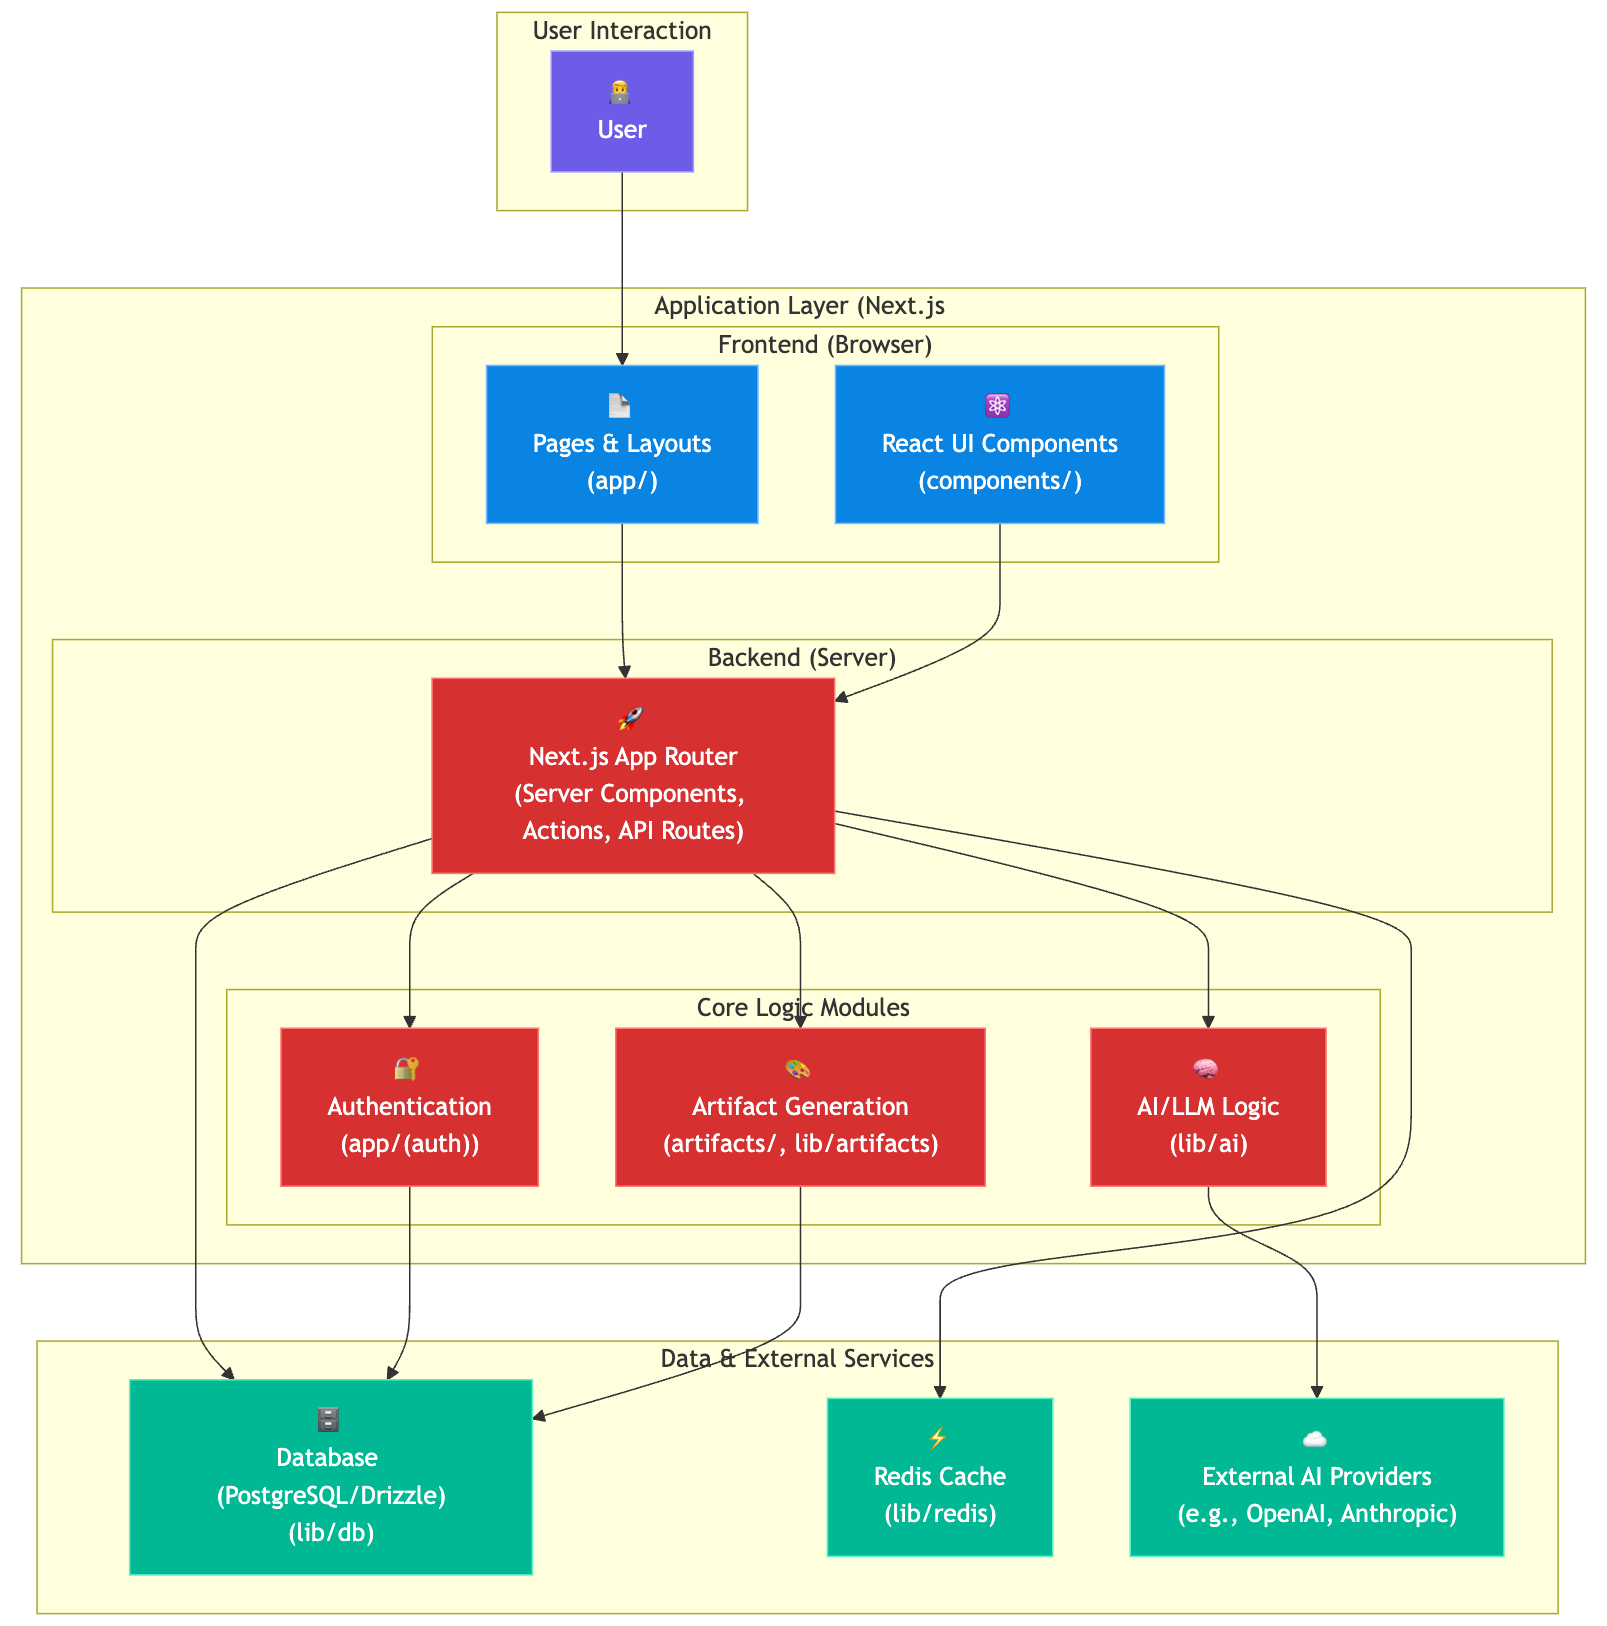
\includegraphics[width=0.9\textwidth]{images/system-arch.png}
  \caption{Arsitektur sistem chatbot dengan RAG dan Langchain}\label{fig:arsitektur-sistem}
\end{figure}

\subsection{Use Case Diagram}
Bagian ini menjelaskan fungsionalitas sistem Chatbot Journal dari perspektif pengguna, yang digambarkan melalui use case diagram. Use case diagram ini mengidentifikasi aktor yang berinteraksi dengan sistem dan berbagai fungsi atau layanan yang disediakan oleh sistem.

\begin{figure}[H]
  \centering
  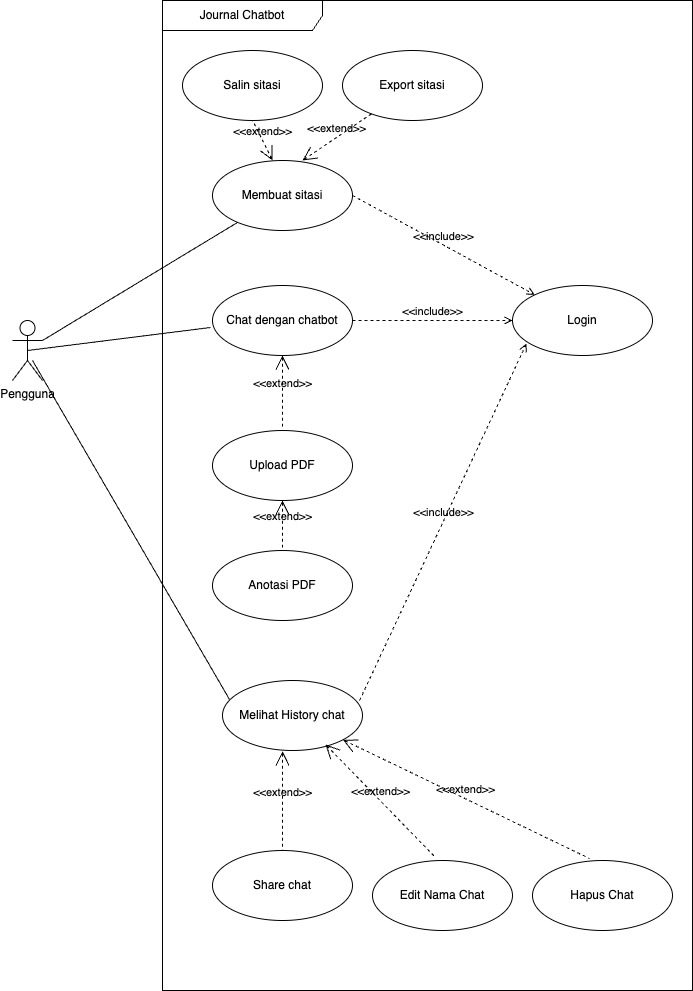
\includegraphics[width=0.9\textwidth]{images/bab-3/usecase.jpg}
  \caption{Use Case Diagram Aplikasi Chatbot Akademik}
  \label{fig:usecase}
\end{figure}
\subsection{Aktor}
Dalam use case diagram ini, terdapat satu aktor utama yaitu \textbf{Pengguna}. Aktor ini merepresentasikan individu yang akan berinteraksi langsung dengan sistem \textit{Journal Chatbot} untuk memenuhi berbagai kebutuhannya terkait manajemen jurnal dan interaksi dengan chatbot.

\subsection{Use Case}
Berikut adalah penjelasan rinci mengenai setiap use case yang terlibat dalam sistem \textit{Journal Chatbot}:

\begin{enumerate}
    \item \textbf{Login}
    \begin{itemize}
        \item \textbf{Deskripsi:} Use case ini memungkinkan pengguna untuk masuk ke dalam sistem dengan menggunakan kredensial yang valid. Ini adalah use case dasar yang harus dilakukan sebelum pengguna dapat mengakses fitur-fitur lain yang memerlukan otentikasi.
        \item \textbf{Relasi:} Use case \textit{Login} di-\textit{include} oleh \textit{Chat dengan Chatbot} dan \textit{Melihat History Chat}, yang berarti setiap kali pengguna ingin melakukan chat atau melihat riwayat chat, mereka harus terlebih dahulu berhasil login.
    \end{itemize}

    \item \textbf{Membuat Sitasi}
    \begin{itemize}
        \item \textbf{Deskripsi:} Use case ini memungkinkan pengguna untuk menghasilkan sitasi dari sumber jurnal atau dokumen yang telah diunggah.
        \item \textbf{Relasi:}
        \begin{itemize}
            \item \textit{Extend Salin Sitasi}: Pengguna dapat memilih untuk menyalin sitasi yang telah dibuat ke clipboard untuk penggunaan lebih lanjut.
            \item \textit{Extend Export Sitasi}: Pengguna dapat memilih untuk mengekspor sitasi ke format lain (misalnya, Bib\TeX, RIS, atau plain text) untuk pengelolaan referensi.
        \end{itemize}
    \end{itemize}

    \item \textbf{Chat dengan Chatbot}
    \begin{itemize}
        \item \textbf{Deskripsi:} Use case ini merupakan inti dari sistem, di mana pengguna dapat berinteraksi secara langsung dengan chatbot untuk mendapatkan informasi, menjawab pertanyaan, atau melakukan tugas-tugas terkait jurnal.
        \item \textbf{Relasi:}
        \begin{itemize}
            \item \textit{Include Login}: Pengguna harus login sebelum dapat berinteraksi dengan chatbot.
            \item \textit{Extend Upload PDF}: Saat berinteraksi dengan chatbot, pengguna memiliki opsi untuk mengunggah dokumen PDF yang kemudian dapat dianalisis atau digunakan oleh chatbot dalam percakapan.
            \item \textit{Extend Anotasi PDF}: Setelah mengunggah PDF, pengguna dapat melakukan anotasi pada dokumen tersebut, seperti menyorot teks, menambahkan catatan, atau menandai bagian-bagian penting. Fitur ini memperkaya interaksi dengan chatbot karena chatbot dapat merujuk pada anotasi pengguna.
        \end{itemize}
    \end{itemize}

    \item \textbf{Melihat History Chat}
    \begin{itemize}
        \item \textbf{Deskripsi:} Use case ini memungkinkan pengguna untuk melihat dan mengelola riwayat percakapan mereka dengan chatbot. Ini sangat penting untuk melacak interaksi sebelumnya dan melanjutkan percakapan.
        \item \textbf{Relasi:}
        \begin{itemize}
            \item \textit{Include Login}: Pengguna harus login untuk dapat mengakses riwayat chat mereka.
            \item \textit{Extend Share Chat}: Pengguna dapat memilih untuk membagikan riwayat chat tertentu dengan pihak lain (misalnya, melalui email atau aplikasi pesan).
            \item \textit{Extend Edit Nama Chat}: Pengguna dapat mengubah nama atau judul dari riwayat chat tertentu untuk mempermudah identifikasi dan pengelolaan.
            \item \textit{Extend Hapus Chat}: Pengguna dapat menghapus riwayat chat yang tidak lagi dibutuhkan untuk menjaga kebersihan data.
        \end{itemize}
    \end{itemize}
\end{enumerate}

\subsection{Relasi Antar Use Case}
\begin{itemize}
    \item \textbf{Relasi \textit{include}}: Menunjukkan bahwa suatu use case menyertakan fungsionalitas dari use case lain secara wajib. Dalam diagram ini, \textit{Login} di-\textit{include} oleh \textit{Chat dengan Chatbot} dan \textit{Melihat History Chat}, yang menekankan bahwa otentikasi adalah prasyarat untuk kedua fungsi tersebut.
    
    \item \textbf{Relasi \textit{extend}}: Menunjukkan bahwa suatu use case dapat memperluas fungsionalitas use case lain dalam kondisi tertentu. Contohnya, \textit{Salin Sitasi} dan \textit{Export Sitasi} adalah opsi tambahan yang tersedia setelah \textit{Membuat Sitasi}. Demikian pula, \textit{Upload PDF} dan \textit{Anotasi PDF} memperluas fungsionalitas \textit{Chat dengan Chatbot}, sementara \textit{Share Chat}, \textit{Edit Nama Chat}, dan \textit{Hapus Chat} memperluas \textit{Melihat History Chat}. Relasi ini menunjukkan fleksibilitas sistem dalam menawarkan fitur tambahan sesuai kebutuhan pengguna.
\end{itemize}

\subsection{Activity Diagram}

Activity Diagram adalah representasi grafis dari alur kerja atau kegiatan di dalam suatu sistem, yang memperlihatkan berbagai langkah yang diperlukan untuk membangun aplikasi chatbot jurnal ini. Berikut merupakan penjelasan lengkap tentang setiap fungsi yang dijalankan sistem ini.

\begin{figure}[H]
  \centering
  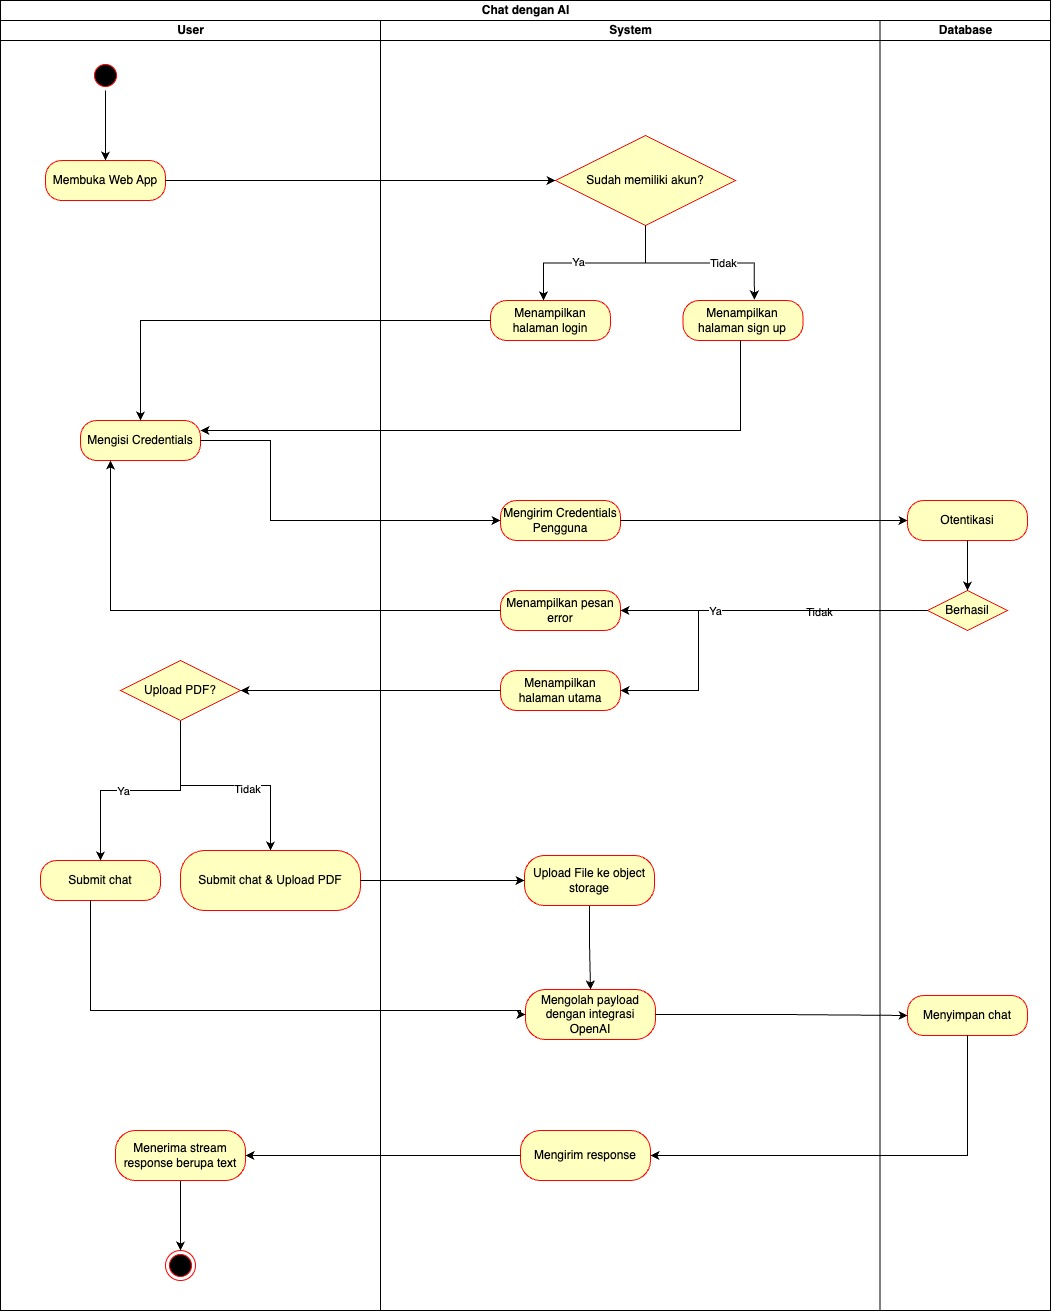
\includegraphics[width=0.9\textwidth]{images/bab-3/sitemap.jpg}
  \caption{Activity Diagram Interaksi Chatbot dengan RAG}
  \label{fig:activity}
\end{figure}

Activity diagram di atas menggambarkan alur proses interaksi pengguna dengan aplikasi. Proses dimulai ketika pengguna membuka web app. Sistem kemudian memeriksa apakah pengguna sudah memiliki akun. Jika belum, sistem akan menampilkan halaman sign up; jika sudah, sistem menampilkan halaman login. Pengguna kemudian mengisi kredensial yang dikirimkan ke sistem untuk proses otentikasi melalui database. Jika otentikasi berhasil, sistem akan menampilkan halaman utama. Jika gagal, sistem akan menampilkan pesan kesalahan.
\singlespacing{}
Setelah berhasil masuk, pengguna dapat memilih apakah ingin mengunggah file PDF atau tidak. Jika tidak, pengguna hanya perlu mengirimkan chat. Namun, jika ingin mengunggah PDF, pengguna akan mengirimkan chat bersamaan dengan file tersebut. File PDF akan diunggah ke object storage, kemudian payload yang berisi chat dan file akan diproses menggunakan integrasi OpenAI.\@ Setelah diproses, hasil response dikirimkan kembali ke sistem dan sistem mengirimkannya ke pengguna dalam bentuk stream teks. Di sisi lain, chat juga disimpan ke dalam database sebagai arsip interaksi.

\subsection{Sequence Diagram}

Gambar~\ref{fig:sequence-login-chat} menunjukkan sequence diagram yang menggambarkan alur interaksi antara pengguna, sistem, dan basis data saat menggunakan aplikasi chatbot jurnal. Diagram ini menjelaskan urutan proses dari mulai membuka aplikasi hingga pengguna menerima respons dari sistem berdasarkan dokumen yang telah diunggah.

\begin{figure}[H]
    \centering
    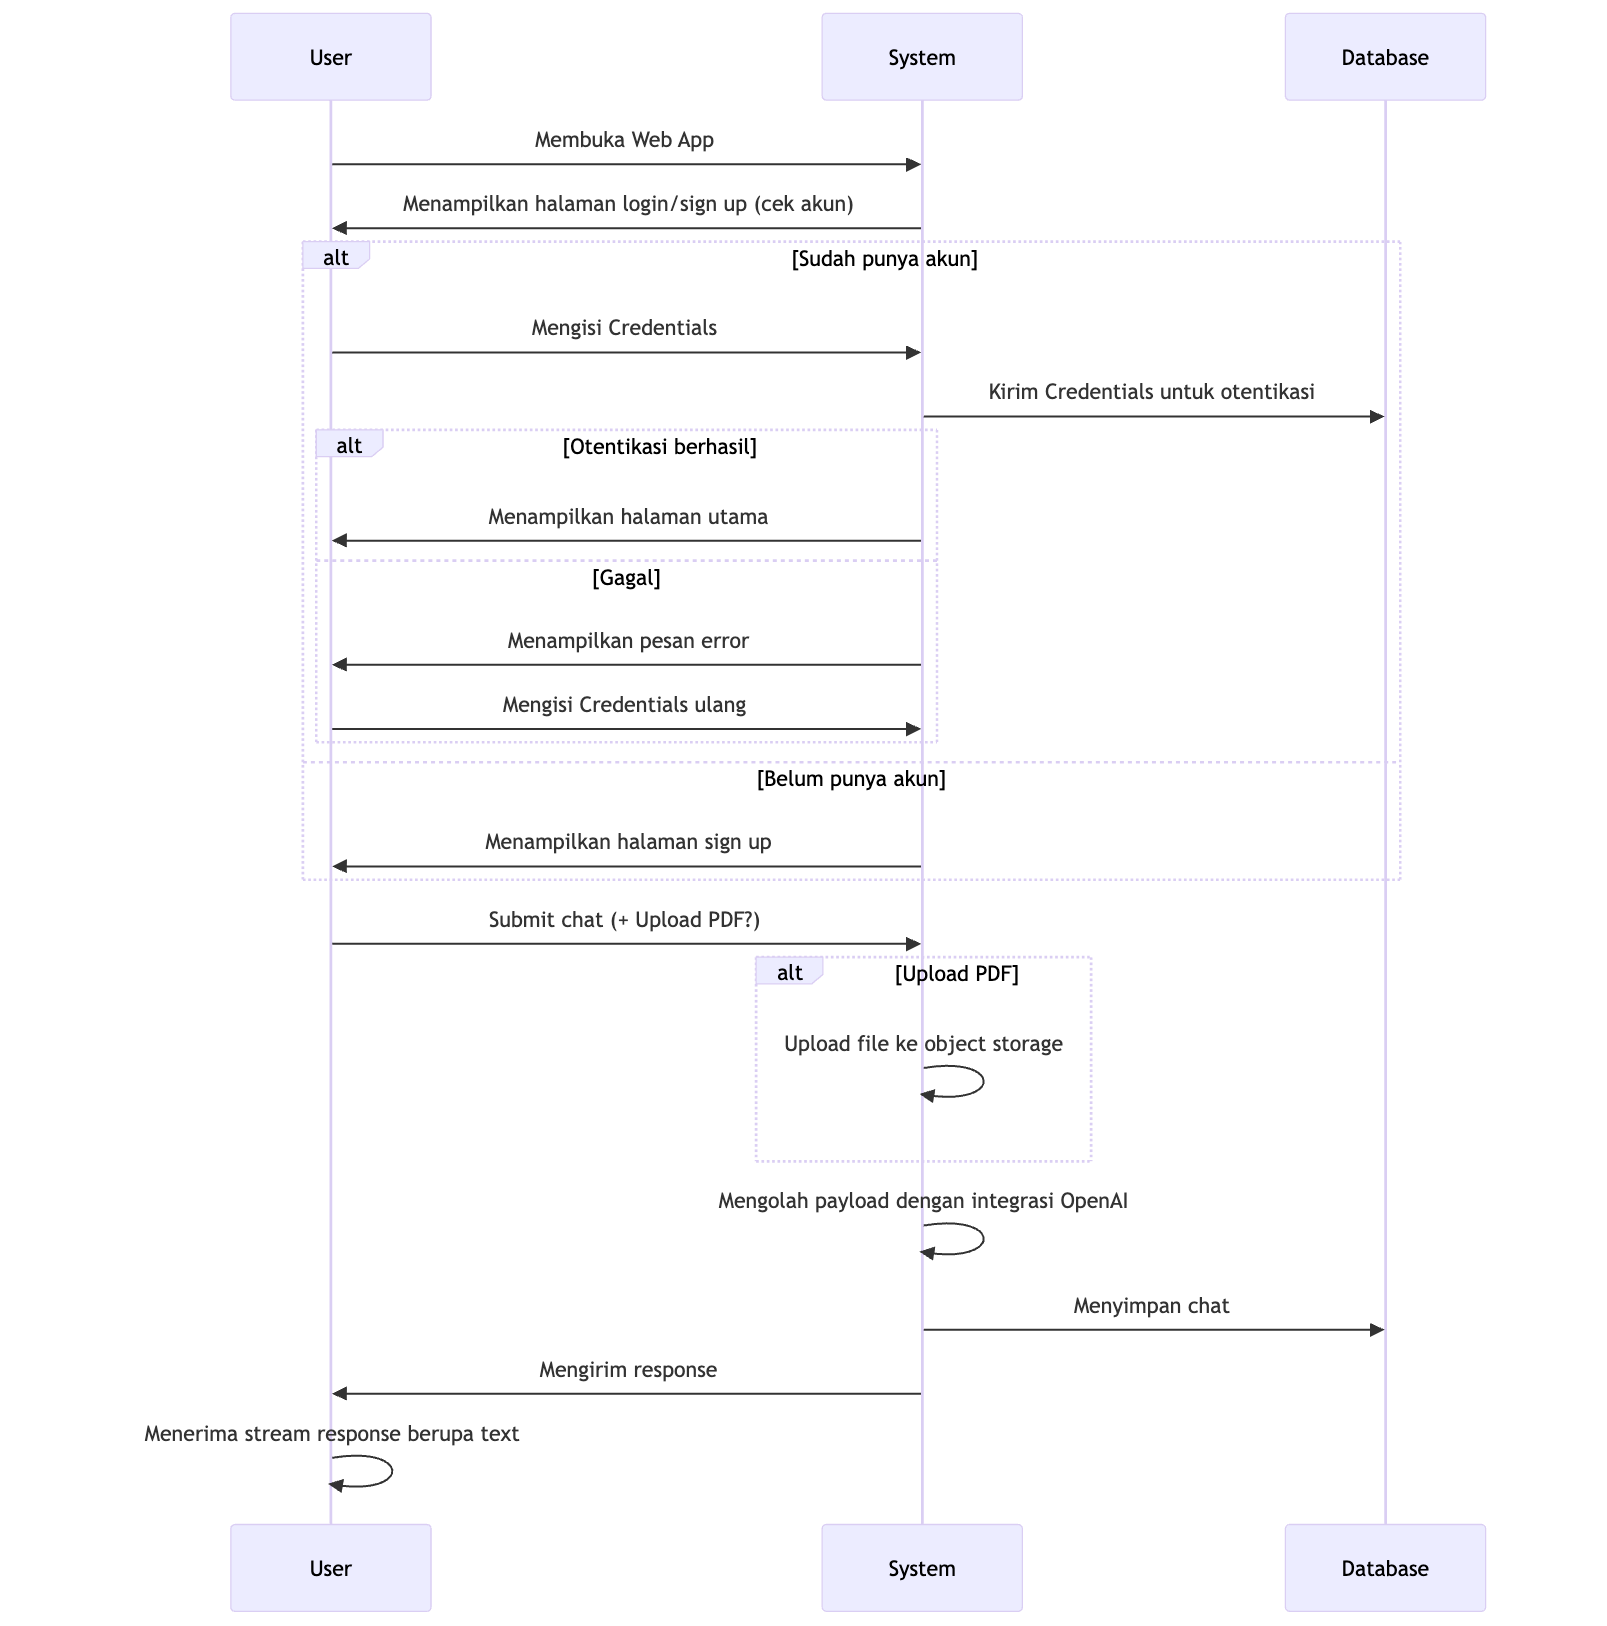
\includegraphics[width=0.9\textwidth]{images/bab-3/sequence.png}
    \caption{Sequence Diagram Interaksi User dan Sistem}
    \label{fig:sequence-login-chat}
\end{figure}

Berdasarkan Gambar~\ref{fig:sequence-login-chat}, berikut adalah tahapan proses yang terjadi:

\begin{enumerate}
  \item \textbf{Pengguna membuka aplikasi web}: Proses dimulai ketika pengguna mengakses aplikasi melalui browser.
  
  \item \textbf{Cek akun dan otentikasi}: Sistem memeriksa apakah pengguna sudah memiliki akun. Jika ya, pengguna mengisi kredensial (email dan password) lalu sistem mengirimkan kredensial tersebut ke backend untuk proses otentikasi.
  
  \item \textbf{Respons otentikasi}: Jika kredensial valid, sistem akan menampilkan halaman utama. Jika tidak, sistem menampilkan pesan error dan meminta pengguna untuk mencoba kembali.
  
  \item \textbf{Registrasi pengguna baru}: Jika pengguna belum memiliki akun, sistem mengarahkan ke halaman sign-up.
  
  \item \textbf{Pengiriman pesan dan dokumen}: Setelah berhasil masuk, pengguna dapat melakukan percakapan dengan chatbot. Jika dibutuhkan, pengguna juga dapat mengunggah file PDF berisi jurnal ilmiah.
  
  \item \textbf{Upload PDF ke Object Storage}: Jika terdapat PDF yang dikirimkan, sistem akan mengunggah file tersebut ke layanan object storage (misalnya Vercel Blob atau storage berbasis cloud lainnya).
  
  \item \textbf{Pemrosesan payload}: Sistem kemudian menggabungkan pertanyaan dan dokumen yang telah diunggah sebagai konteks untuk dikirim ke model LLM (OpenAI GPT-4) melalui integrasi Langchain.
  
  \item \textbf{Penyimpanan riwayat chat}: Setelah mendapatkan hasil respons dari model AI, sistem menyimpan riwayat percakapan (chat) ke basis data untuk kepentingan histori pengguna.
  
  \item \textbf{Streaming respons ke pengguna}: Respons dari model dikirimkan secara bertahap dalam bentuk streaming teks ke pengguna, untuk pengalaman percakapan yang lebih cepat dan real-time.
\end{enumerate}

Diagram ini memvisualisasikan bagaimana sistem menangani proses otentikasi, pengelolaan dokumen, dan integrasi dengan layanan AI secara terstruktur dan efisien. Alur ini juga menunjukkan bahwa sistem bersifat stateless pada sisi server, karena menggunakan pendekatan API tanpa backend server monolitik.

\subsection{Entity Relationship Diagram (ERD)}

Entity Relationship Diagram (ERD) digunakan untuk menggambarkan struktur dan relasi antar tabel dalam basis data aplikasi chatbot berbasis \textit{Retrieval-Augmented Generation (RAG)}. Diagram ini membantu dalam merancang basis data yang efisien dan sesuai dengan kebutuhan fungsional aplikasi.

\begin{figure}[H]
  \centering
  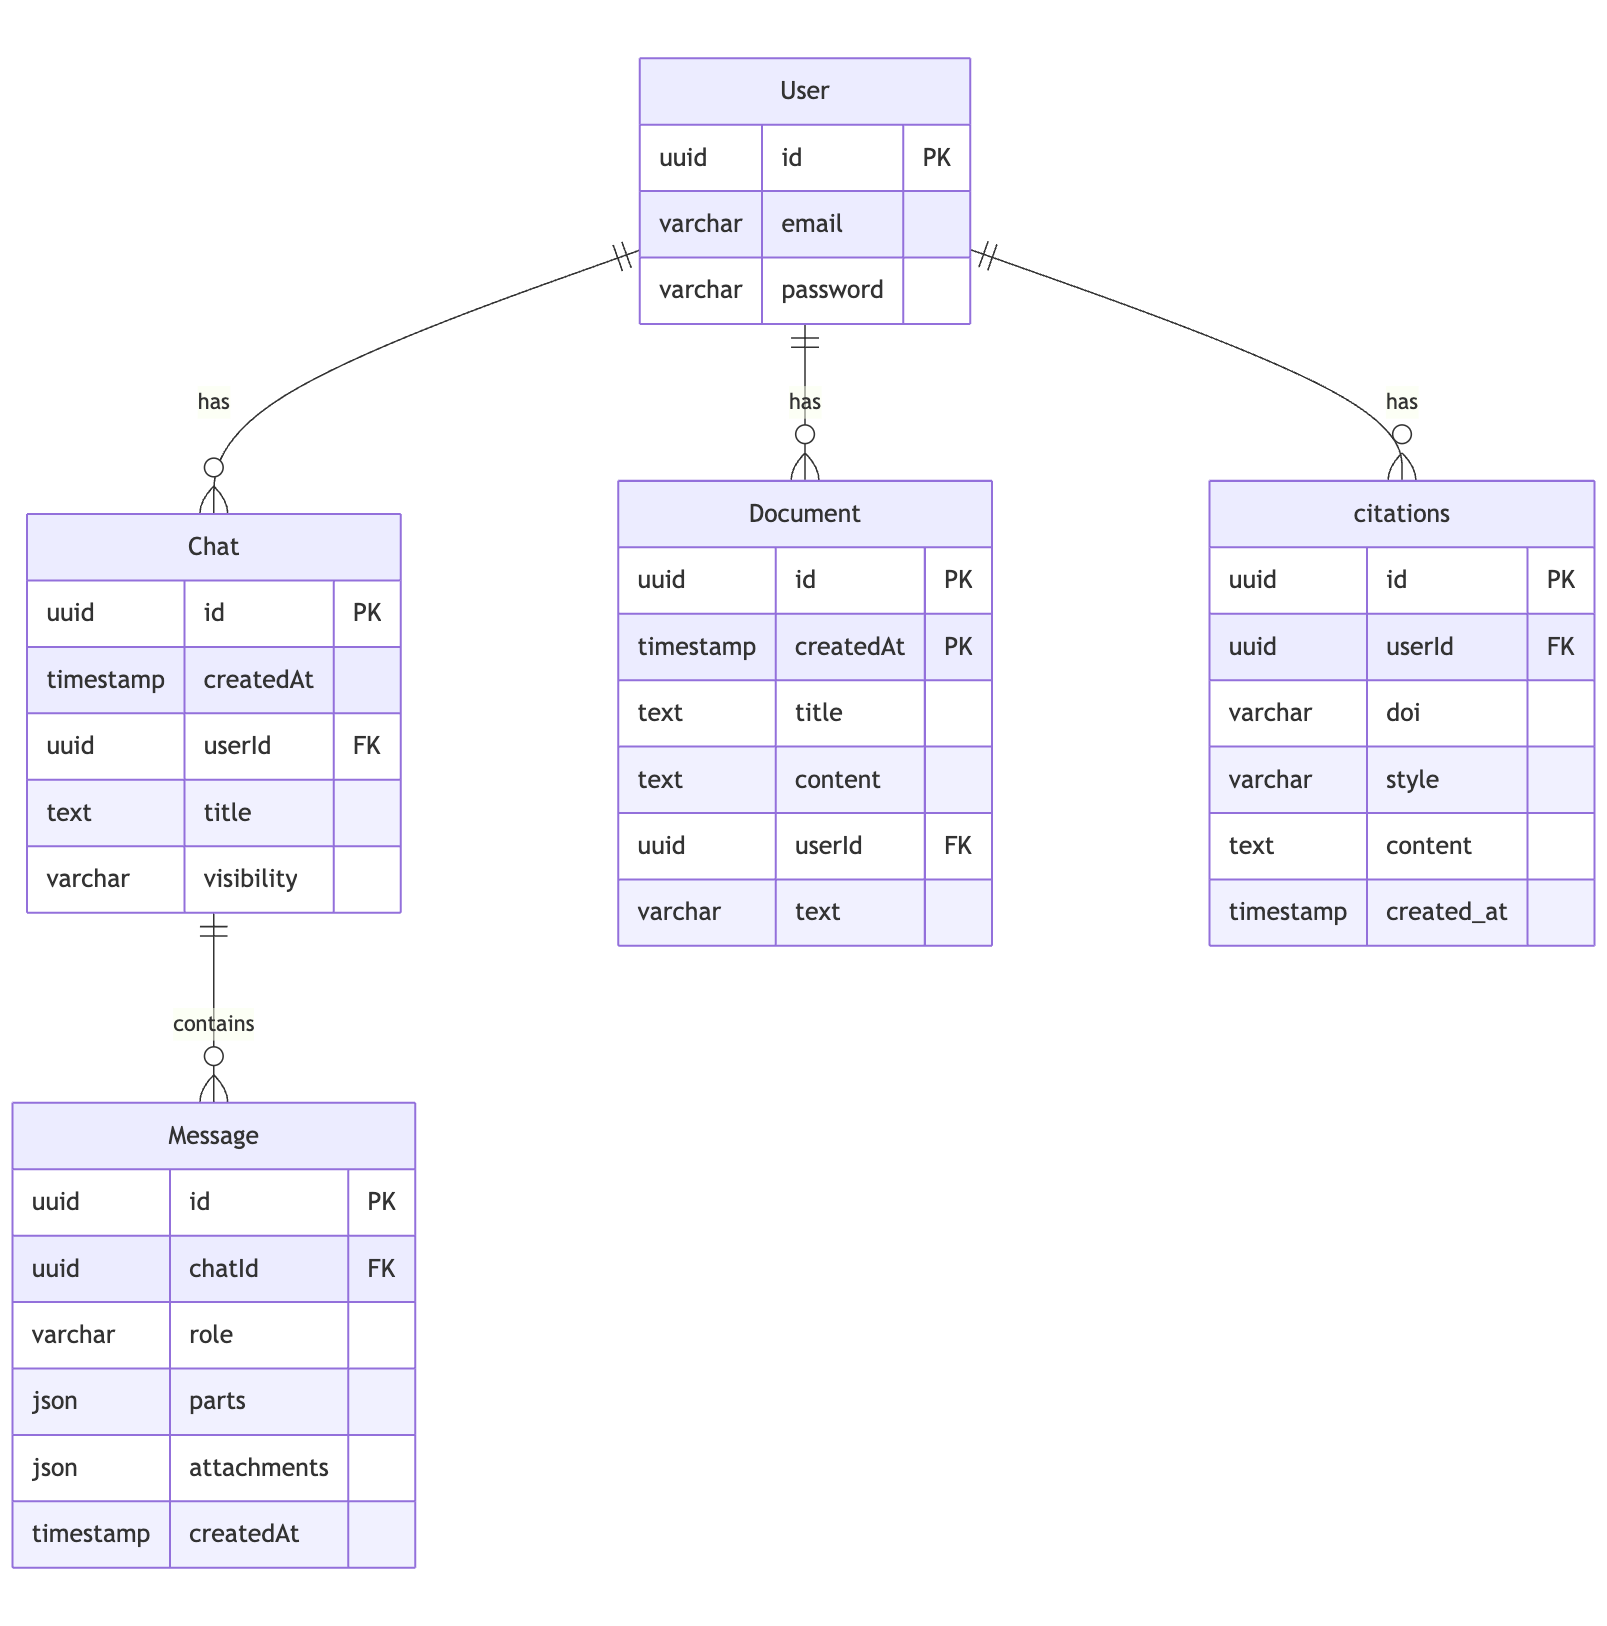
\includegraphics[width=0.95\linewidth]{images/bab-3/erd-skripsi.png}
  \caption{Entity Relationship Diagram Aplikasi}
  \label{fig:erd}
\end{figure}

\noindent Penjelasan masing-masing entitas dalam ERD adalah sebagai berikut:

\begin{itemize}
  \item \textbf{User} \\
  Entitas \texttt{User} menyimpan data pengguna yang terautentikasi. Atribut yang dimiliki:
  \begin{itemize}
    \item \texttt{id}: UUID sebagai \textit{primary key}
    \item \texttt{email}: Alamat email pengguna
    \item \texttt{password}: Kata sandi pengguna (dalam bentuk terenkripsi)
  \end{itemize}
  Relasi: Satu pengguna dapat memiliki banyak \texttt{Chat}, \texttt{Document}, dan \texttt{Citations}.

  \item \textbf{Chat} \\
  Entitas ini merepresentasikan sesi percakapan antara pengguna dan sistem chatbot. Atribut:
  \begin{itemize}
    \item \texttt{id}: UUID sebagai \textit{primary key}
    \item \texttt{createdAt}: Timestamp waktu pembuatan chat
    \item \texttt{userId}: FK mengacu ke \texttt{User}
    \item \texttt{title}: Judul percakapan
    \item \texttt{visibility}: Status visibilitas percakapan (privat/publik)
  \end{itemize}
  Relasi: Satu \texttt{Chat} memiliki banyak \texttt{Message}.

  \item \textbf{Message} \\
  Menyimpan seluruh pesan yang terkandung dalam satu sesi chat. Atribut:
  \begin{itemize}
    \item \texttt{id}: UUID sebagai \textit{primary key}
    \item \texttt{chatId}: FK ke \texttt{Chat}
    \item \texttt{role}: Peran pengirim pesan (user/system)
    \item \texttt{parts}: Konten pesan dalam format JSON
    \item \texttt{attachments}: Lampiran terkait dalam format JSON
    \item \texttt{createdAt}: Timestamp pembuatan pesan
  \end{itemize}

  \item \textbf{Document} \\
  Entitas ini menyimpan data dokumen PDF yang diunggah oleh pengguna. Atribut:
  \begin{itemize}
    \item \texttt{id}: UUID sebagai \textit{primary key}
    \item \texttt{createdAt}: Waktu unggahan dokumen
    \item \texttt{title}: Judul dokumen
    \item \texttt{content}: Isi teks hasil ekstraksi PDF
    \item \texttt{userId}: FK ke \texttt{User}
    \item \texttt{text}: Versi teks tambahan atau metadata (opsional)
  \end{itemize}

  \item \textbf{Citations} \\
  Menyimpan kutipan atau sitasi yang dibuat pengguna berdasarkan dokumen yang telah diunggah. Atribut:
  \begin{itemize}
    \item \texttt{id}: UUID sebagai \textit{primary key}
    \item \texttt{userId}: FK ke \texttt{User}
    \item \texttt{doi}: Digital Object Identifier dari jurnal
    \item \texttt{style}: Gaya kutipan (APA, IEEE, Harvard, dll)
    \item \texttt{content}: Format sitasi lengkap
    \item \texttt{created\_at}: Waktu pembuatan sitasi
  \end{itemize}
\end{itemize}
\section{Implementasi Sistem}

Tahap implementasi merupakan proses penting dalam membangun aplikasi sesuai rancangan dan spesifikasi teknis. Sistem ini dikembangkan menggunakan pendekatan \textit{fullstack} dengan framework Next.js 15 (App Router) dan database PostgreSQL yang dihosting melalui layanan Neon. Tidak ada \textit{back-end} terpisah, seluruh \textit{server logic} ditulis dalam API Routes di dalam struktur Next.js. Implementasi juga melibatkan integrasi Langchain, Retrieval-Augmented Generation (RAG), OpenAI API, serta fitur anotasi PDF menggunakan PDF.js. Berikut adalah langkah-langkah implementasi yang dilakukan:

\subsection{Persiapan Database PostgreSQL (Neon)}

\begin{itemize}
  \item Membuat akun dan proyek baru di \url{https://neon.tech}, kemudian membuat \texttt{branch}, \texttt{database}, dan \texttt{user}.
  \item Menyimpan kredensial \texttt{host}, \texttt{database}, \texttt{user}, dan \texttt{password} ke dalam file \texttt{.env} proyek.
  \item Menyusun skema database berdasarkan ERD menggunakan perintah SQL secara manual.
  \item Tabel-tabel utama meliputi: \texttt{users}, \texttt{chats}, \texttt{messages}, \texttt{documents}, dan \texttt{citations}.
\end{itemize}

\subsection{Inisialisasi Proyek Next.js 15}

\begin{itemize}
  \item Menginisialisasi proyek dengan perintah:
  \begin{verbatim}
  npx create-next-app@latest ai-journal-assistant --typescript --app
  \end{verbatim}
  \item Mengaktifkan Tailwind CSS dan PostCSS untuk styling antarmuka.
  \item Menyiapkan folder \texttt{app/api/} untuk menyimpan seluruh logika server-side.
\end{itemize}

\subsection{Integrasi Langchain dan RAG}

\begin{itemize}
  \item Menginstal dependensi utama:
  \begin{verbatim}
  npm install langchain @langchain/community @langchain/openai
  \end{verbatim}
  \item Menggunakan pipeline \texttt{RetrievalQAChain} dari Langchain untuk menghubungkan retriever dan model LLM (GPT-4).
  \item Langkah-langkah implementasi:
  \begin{itemize}
    \item Mengekstrak teks dari PDF.\@
    \item Memecah teks menjadi potongan pendek (\texttt{text splitting}).
    \item Membuat embeddings dengan model dari OpenAI (\texttt{text-embedding-ada-002}).
    \item Menyimpan embeddings ke dalam \texttt{vector store} (menggunakan Chroma).
    \item Melakukan similarity search ketika pengguna mengajukan pertanyaan.
    \item Menyediakan jawaban dari LLM yang memperhitungkan hasil retrieval.
  \end{itemize}
\end{itemize}

\subsection{Integrasi OpenAI API}

\begin{itemize}
  \item Mengatur API Key di \texttt{.env} sebagai \texttt{OPENAI\_API\_KEY}.
  \item Menggunakan endpoint \texttt{/api/chat} untuk menerima \texttt{prompt} dan merespons dengan hasil dari GPT-4.
  \item Mendukung konteks percakapan dengan menyimpan riwayat \texttt{messages} pada database.
\end{itemize}

\subsection{Penyimpanan Dokumen PDF dengan Vercel Blob}

\begin{itemize}
  \item Menggunakan \texttt{@vercel/blob} untuk menyimpan file PDF dari pengguna secara langsung ke storage Vercel.
  \item File PDF ini kemudian diakses kembali oleh sistem untuk proses ekstraksi isi dokumen.
  \item URL dokumen disimpan pada tabel \texttt{documents} dalam database.
\end{itemize}

\subsection{Manajemen State dan Cache dengan Redis (Upstash)}
\begin{itemize}
  \item Menggunakan Redis sebagai cache session dan penyimpanan embeddings sementara.
  \item Mendaftar ke layanan \url{https://upstash.com} dan menambahkan variabel \texttt{UPSTASH\_REDIS\_URL} dan \texttt{TOKEN} pada \texttt{.env}.
  \item Menggunakan package \texttt{@upstash/redis} untuk operasi Redis dalam API Routes.
\end{itemize}

\subsection{Preview dan Anotasi PDF dengan PDF.js}
\begin{itemize}
  \item Mengintegrasikan \texttt{pdfjs-dist} untuk menampilkan dokumen PDF secara langsung di browser.
  \item Fitur anotasi dikembangkan dengan menambahkan layer interaktif di atas canvas, yang mencatat teks yang dipilih dan menampilkan input komentar.
  \item Catatan dan posisi anotasi disimpan dalam tabel \texttt{annotations} atau bagian dari \texttt{documents}.
\end{itemize}
\section{Implementasi Fitur Utama}
\subsection{Upload dan Pratinjau PDF}
Pengguna dapat mengunggah file PDF yang akan disimpan pada \texttt{Vercel Blob}. File ini kemudian dimuat dan dipratinjau menggunakan \texttt{PDF.js}.
\begin{lstlisting}[language=TypeScript, caption={Chat dengan AI}]
'use client';

import { ChatHeader } from '@/components/chat-header';
import { useArtifactSelector } from '@/hooks/use-artifact';
import type { Vote } from '@/lib/db/schema';
import { fetcher, generateUUID } from '@/lib/utils';
import { useChat } from '@ai-sdk/react';
import type { Attachment, UIMessage } from 'ai';
import type { Session } from 'next-auth';
import { useRouter, useSearchParams } from 'next/navigation';
import { useEffect, useRef, useState } from 'react';
import useSWR, { useSWRConfig } from 'swr';
import { unstable_serialize } from 'swr/infinite';
import { Artifact } from './artifact';
import { Messages } from './messages';
import { MultimodalInput } from './multimodal-input';
import { getChatHistoryPaginationKey } from './sidebar-history';
import { toast } from './toast';
import type { VisibilityType } from './visibility-selector';

import dynamic from 'next/dynamic';
const PDFViewer = dynamic(() => import('../components/pdf-viewer'), {
  ssr: false,
});

import { Show } from './shared/show';
import { useBoolean } from '@/hooks/use-boolean';
import { useMediaQuery } from 'usehooks-ts';

export function Chat({
  id,
  initialMessages,
  selectedChatModel,
  selectedVisibilityType,
  isReadonly,
  session,
  attachmentUrl,
}: {
  id: string;
  initialMessages: Array<UIMessage>;
  selectedChatModel: string;
  selectedVisibilityType: VisibilityType;
  isReadonly: boolean;
  session: Session;
  attachmentUrl?: string;
}) {
  const { mutate } = useSWRConfig();
  const isPDFSubmitted = useRef(false);
  const router = useRouter();

  const {
    messages,
    setMessages,
    handleSubmit,
    input,
    setInput,
    append,
    status,
    stop,
    reload,
  } = useChat({
    id,
    initialMessages,
    experimental_throttle: 100,
    sendExtraMessageFields: true,
    generateId: generateUUID,
    experimental_prepareRequestBody: (body) => ({
      id,
      message: body.messages.at(-1),
      selectedChatModel,
    }),
    onFinish: () => {
      mutate(unstable_serialize(getChatHistoryPaginationKey));
    },
    onResponse: () => {
      if (isPDFSubmitted.current) return;
      isPDFSubmitted.current = true;
      router.refresh();
      return;
    },
    onError: (error) => {
      toast({
        type: 'error',
        description: error.message,
      });
    },
  });

  const searchParams = useSearchParams();
  const query = searchParams.get('query');

  const [hasAppendedQuery, setHasAppendedQuery] = useState(false);

  useEffect(() => {
    if (query && !hasAppendedQuery) {
      append({
        role: 'user',
        content: query,
      });

      setHasAppendedQuery(true);
      window.history.replaceState({}, '', `/chat/${id}`);
    }
  }, [query, append, hasAppendedQuery, id]);

  const { data: votes } = useSWR<Array<Vote>>(
    messages.length >= 2 ? `/api/vote?chatId=${id}` : null,
    fetcher,
  );

  const [attachments, setAttachments] = useState<Array<Attachment>>([]);
  const { value: isPdfVisible, toggle: togglePdfVisible } = useBoolean(true);
  const isArtifactVisible = useArtifactSelector((state) => state.isVisible);
  const isMobile = useMediaQuery('(max-width: 1024px)');

  return (
    <>
      <div
        className={`flex flex-col min-w-0 h-dvh bg-background ${
          attachmentUrl ? 'md:flex-row' : ''
        }`}
      >
        <div
          className={`flex flex-col flex-1 ${attachmentUrl ? 'md:w-1/2' : 'w-full'}`}
        >
          <ChatHeader
            chatId={id}
            selectedModelId={selectedChatModel}
            selectedVisibilityType={selectedVisibilityType}
            isReadonly={isReadonly}
            session={session}
            isPdfVisible={isPdfVisible}
            onPdfToggle={togglePdfVisible}
            showPdfToggle={Boolean(attachmentUrl)}
          />

          {/* mobile pdf viewer */}
          <Show
            when={
              Boolean(attachmentUrl) &&
              attachmentUrl !== '' &&
              isPdfVisible &&
              isMobile
            }
          >
            <PDFViewer chatId={id} url={attachmentUrl as string} />
          </Show>

          <Messages
            chatId={id}
            status={status}
            votes={votes}
            messages={messages}
            setMessages={setMessages}
            reload={reload}
            isReadonly={isReadonly}
            isArtifactVisible={isArtifactVisible}
          />

          <form className="flex mx-auto px-4 bg-background pb-4 md:pb-6 gap-2 w-full md:max-w-3xl">
            <Show when={!isReadonly}>
              <MultimodalInput
                chatId={id}
                input={input}
                setInput={setInput}
                handleSubmit={handleSubmit}
                status={status}
                stop={stop}
                attachments={attachments}
                setAttachments={setAttachments}
                messages={messages}
                setMessages={setMessages}
                append={append}
              />
            </Show>
          </form>
        </div>

        <Show
          when={
            Boolean(attachmentUrl) &&
            attachmentUrl !== '' &&
            isPdfVisible &&
            !isMobile
          }
        >
          <div className="flex-1 md:w-1/2 overflow-y-auto bg-gray-100">
            <PDFViewer chatId={id} url={attachmentUrl as string} />
          </div>
        </Show>
      </div>

      <Artifact
        chatId={id}
        input={input}
        setInput={setInput}
        handleSubmit={handleSubmit}
        status={status}
        stop={stop}
        attachments={attachments}
        setAttachments={setAttachments}
        append={append}
        messages={messages}
        setMessages={setMessages}
        reload={reload}
        votes={votes}
        isReadonly={isReadonly}
      />
    </>
  );
}
\end{lstlisting}

\subsection{Tanya Jawab Berbasis RAG}
Sistem menggunakan pipeline \texttt{Langchain} untuk menjalankan \textit{Retrieval-Augmented Generation}:
\begin{enumerate}
  \item Ekstraksi teks dari PDF
  \item Pemecahan menjadi chunk dengan overlap
  \item Embedding menggunakan model dari \texttt{OpenAI API}
  \item Penyimpanan dalam vektor menggunakan \texttt{ChromaDB}
  \item Retrieval saat tanya jawab berdasarkan \texttt{cosine similarity}
  \item Prompt otomatis digabung dengan hasil retrieval dan dikirim ke model GPT
\end{enumerate}

\subsection{Retrieval-Augmented Generation}
Agar LLM dapat bekerja dengan dokumen pribadi seperti PDF, konten dokumen harus diproses dan disimpan dengan cara yang dapat diakses secara efisien oleh LLM.\@ Seluruh proses ini dikenal sebagai \emph{ingestion} \citep[p~.84]{oshin2024learning}. Ide intinya adalah mengubah teks menjadi representasi numerik yang disebut \emph{embeddings} dan menyimpannya dalam penyimpanan \emph{vektor store} (sejenis basis data vektor). Hal ini memungkinkan aplikasi untuk menemukan dan mengambil bagian yang paling relevan dari dokumen untuk menjawab pertanyaan spesifik pengguna. Proses ini melibatkan empat langkah utama:
\begin{enumerate}
  \item \emph{Loading}: Mengekstrak teks dari dokumen PDF.
  \item \emph{Splitting}: Memecah teks yang diekstrak menjadi bagian yang lebih kecil dan mudah dikelola.
  \item \emph{Embedding}: Mengubah setiap potongan teks menjadi vektor numerik yang menangkap makna semantiknya.
  \item \emph{Storing}: Menyimpan \emph{embeddings} ini dalam penyimpanan vektor untuk pencarian yang efisien.
\end{enumerate}

\begin{figure}[htbp]
  \centering
  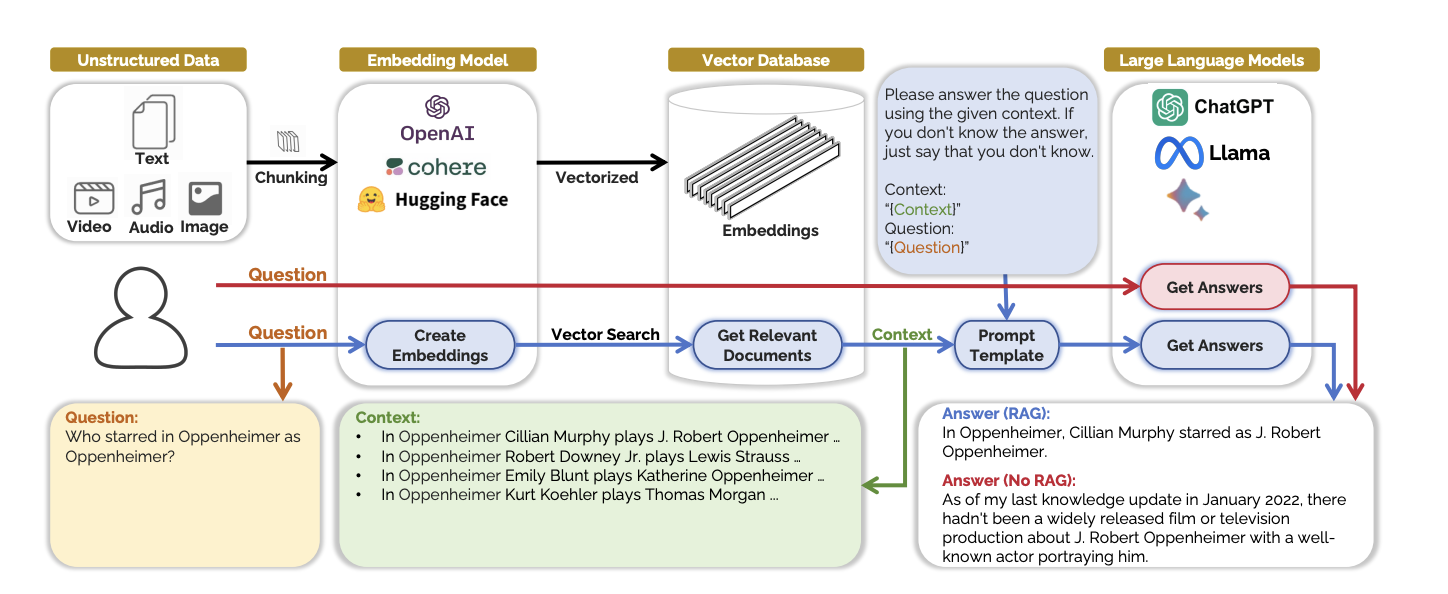
\includegraphics[width=0.85\linewidth]{images/bab-3/embeddings.png}
  \caption{Contoh \emph{RAG framework} yang menggunakan \emph{Vector Database}.}\label{fig:RAG-Framework}\citep{Jing}
\end{figure}

\subsection{Pembuatan Sitasi Otomatis}
Sistem melakukan ekstraksi metadata seperti judul, penulis, tahun, dan DOI dari PDF dan menyusunnya ke dalam format referensi (APA, MLA, IEEE, Harvard) secara otomatis.

\subsection{Anotasi PDF}
Menggunakan integrasi \texttt{PDF.js}, pengguna dapat melakukan:
\begin{itemize}
  \item Highlight teks
  \item Menambahkan catatan
  \item Menyimpan anotasi ke database untuk ditampilkan ulang
\end{itemize}
\section{Teknik Pengumpulan dan Analisis Data}
Data yang dikumpulkan mencakup interaksi pengguna dengan sistem, log respons chatbot, dan hasil uji coba fungsionalitas. Teknik pengumpulan data dilakukan melalui:
\begin{itemize}
  \item \textbf{Observasi langsung} saat pengguna menguji aplikasi.
  \item \textbf{Log sistem} untuk merekam performa model dan hasil pencarian RAG.
  \item \textbf{Kuesioner} untuk mengevaluasi aspek usability dari sisi pengguna.
\end{itemize}

\section{Pengujian dan Evaluasi}
Setiap iterasi diuji dengan pendekatan:
\begin{itemize}
  \item \textbf{Pengujian fungsional} untuk memastikan seluruh fitur seperti upload, tanya jawab, sitasi, dan anotasi bekerja sebagaimana mestinya.
  \item \textbf{Evaluasi usability} melalui uji coba langsung oleh pengguna sasaran (mahasiswa) untuk mendapatkan umpan balik terkait kemudahan dan efektivitas penggunaan sistem.
\end{itemize}
\section{Deployment dan Pengujian Aplikasi}

\begin{itemize}
  \item Aplikasi di-deploy ke \texttt{Vercel} dengan environment variables yang dikonfigurasi langsung di dashboard.
  \item Database Neon dan Redis Upstash beroperasi sebagai layanan terpisah dan dihubungkan melalui koneksi aman.
  \item Pengujian dilakukan melalui \texttt{functional testing} dan \texttt{usability testing} untuk memastikan semua fitur berjalan sesuai tujuan awal.
\end{itemize}

\noindent
Dengan mengikuti alur implementasi di atas, sistem chatbot dapat berjalan sesuai \emph{requirements} dan terintegrasi penuh antara penyimpanan dokumen, pencarian berbasis vektor, dan generasi jawaban kontekstual melalui LLM.
\chapter{HASIL DAN PEMBAHASAN}

\section{Hasil...}
Bab ini membahas hasil implementasi dan evaluasi dari sistem aplikasi chatbot berbasis jurnal ilmiah yang dikembangkan menggunakan pendekatan \textit{Retrieval-Augmented Generation} (RAG) dengan dukungan framework \textit{Langchain}. Sistem ini dibangun menggunakan \texttt{Next.js 15 App Router} dan \texttt{TypeScript} pada sisi \textit{front-end}, \texttt{PostgreSQL} untuk basis data, \texttt{OpenAI API} untuk layanan LLM, serta \texttt{Vercel Blob} untuk menyimpan file PDF yang diunggah. Sistem ini juga mengintegrasikan \texttt{PDF.js} untuk pratinjau dan anotasi PDF secara langsung di antarmuka pengguna.

\section{Pembahasan}

\subsection{Efektivitas RAG dan Langchain}
Integrasi RAG dengan Langchain memungkinkan sistem memberikan jawaban yang lebih akurat dan kontekstual, terutama pada jurnal yang panjang. Proses retrieval meminimalisasi kesalahan faktual karena model hanya bekerja berdasarkan informasi dari dokumen.

\subsection{Evaluasi Pengguna}
Uji coba dilakukan dengan 10 pengguna yang merupakan mahasiswa. Mayoritas menyatakan fitur chatbot dan anotasi membantu mereka memahami jurnal lebih baik. Pembuatan sitasi otomatis juga mempercepat proses penulisan.

\subsection{Kelebihan dan Keterbatasan}
\begin{itemize}
  \item \textbf{Kelebihan:} Akurasi tinggi, UI intuitif, dan kemampuan anotasi.
  \item \textbf{Keterbatasan:} Performa retrieval bergantung pada struktur PDF, dan sistem belum mendukung pertanyaan multipdf.
\end{itemize}

\section{Ringkasan}
Bab ini telah memaparkan hasil implementasi sistem, mulai dari arsitektur, rancangan diagram, implementasi fitur utama, hingga pembahasan efektivitas sistem yang dikembangkan. Evaluasi menunjukkan bahwa aplikasi dapat membantu pengguna dalam memahami jurnal dan membuat sitasi dengan lebih efisien.
\chapter{PENUTUP}

\section{Kesimpulan}

Secara keseluruhan, penelitian ini berhasil menghasilkan model klasifikasi
\emph{deepfake} yang efektif dan aplikasi web yang interaktif, serta
memenuhi kriteria keberhasilan yang telah dipaparkan pada bagian Pemahaman
Bisnis. Hasil ini penting untuk meningkatkan kinerja model dalam mengklasifikasi
\emph{deepfake} di masa mendatang dan memberikan alat yang berguna
bagi masyarakat untuk mengidentifikasi \emph{deepfake}. Meskipun demikian,
penelitian lebih lanjut diperlukan untuk terus meningkatkan kinerja
model dan mengeksplorasi teknik dan pendekatan baru dalam pengklasifikasian
\emph{deepfake}.

\section{Saran}

Berdasarkan hasil penelitian dan pengujian yang telah dilakukan, berikut adalah beberapa saran untuk penelitian dan pengembangan lebih lanjut dalam bidang klasifikasi dan deteksi \emph{deepfake} pada gambar dan/atau video singkat:
\clearpage 
\phantomsection 
\renewcommand\bibname{DAFTAR PUSTAKA}\bibliographystyle{apalike}
\addcontentsline{toc}{chapter}{\bibname}\bibliography{biblio}


\chapter*{LAMPIRAN}

\setcounter{page}{1}
\appendixpagenumbering
\thispagestyle{appendixstyle}
\pagestyle{appendixstyle}
\addcontentsline{toc}{chapter}{LAMPIRAN}

\section*{Lampiran 1 \emph{Dataset}}

\addcontentsline{app}{appendices}{Lampiran 1 \textit{Dataset}}

\subsection*{Ukuran \emph{Dataset}}
\begin{center}
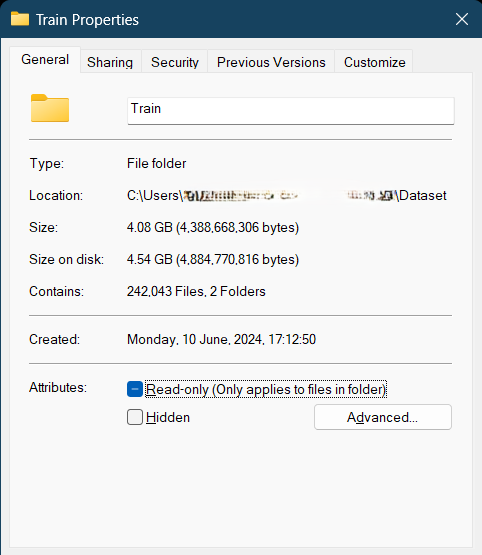
\includegraphics[width=4.55cm]{images/prop_train} 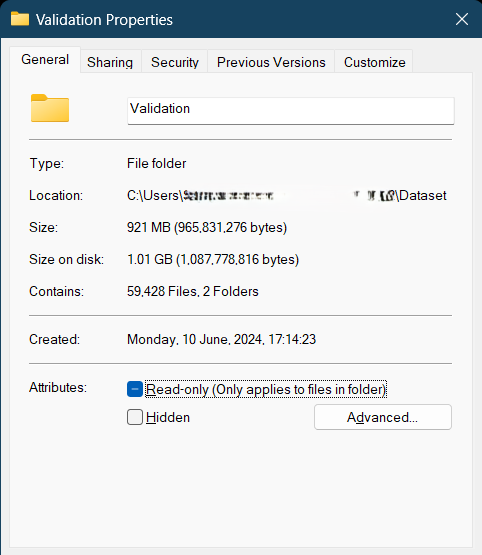
\includegraphics[width=4.55cm]{images/prop_valid}
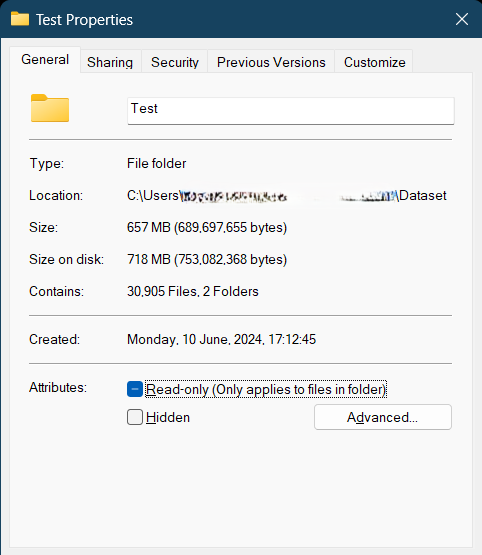
\includegraphics[width=4.55cm]{images/prop_test}
\par\end{center}

\clearpage
\phantomsection

\section*{Lampiran 2 Jupyter Notebook}

\addcontentsline{app}{appendices}{Lampiran 2 Jupyter Notebook}

\subsection*{Arsitektur Model}
\begin{center}
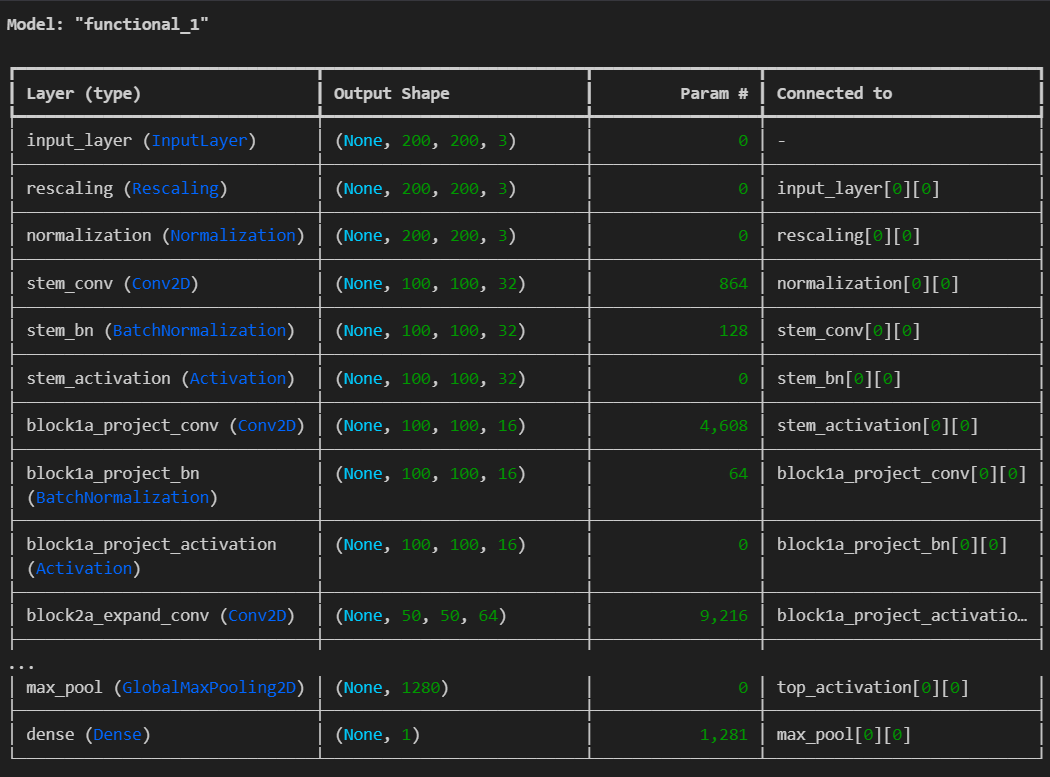
\includegraphics[width=14cm]{images/model_1}
\par\end{center}

\subsection*{pi24\_train.ipynb}

\begin{lstlisting}[numbers=left,basicstyle={\tiny},breaklines=true,showstringspaces=false,tabsize=5]
import numpy as np 
import tensorflow as tf 
import os import keras 
from tensorflow.keras.preprocessing.image import ImageDataGenerator, img_to_array, load_img 
from tensorflow.keras.applications import EfficientNetV2B0 
from tensorflow.keras.layers import Dense 
from tensorflow.keras.models import Model 
from tensorflow.keras.optimizers import Adam 
import matplotlib.pyplot as plt
\end{lstlisting}

\clearpage
\phantomsection
\end{document}
